\documentclass[11pt]{article}
\usepackage[a4paper,margin=24mm]{geometry}
\usepackage{amsmath,amssymb,mathtools,amsthm,mathrsfs,tikz,longtable,booktabs,array,calc,enumitem}
\usepackage[hidelinks,hypertexnames=false]{hyperref}\usepackage{xurl}
\usepackage{fontspec}\setmainfont{DejaVu Serif}
\usetikzlibrary{arrows.meta,positioning}
\setlength{\emergencystretch}{3em}\providecommand{\tightlist}{}
\title{Original inverse-sector quotients:\\source shifts, heat and covariance angles}
\author{Split-Zero research programme}\date{21 September 2026\\SZ-20260921-013}
\begin{document}\maketitle
The original inverse-power space can be removed through explicit maps of
the observation complex, with its complete minimum metric and source
relations retained. The kernel determinant changes by $o(kq)$ on the
stated original degree regime; multiplication by $y^r$ identifies the
result with a full polynomial source at the displayed shifted cutoff.

The coefficient of the retained observed inverse-power determinant is
exactly the older $C_\partial$. The equality below preserves all elliptic
constants. A new bound controls the quotient angle under the full source
covariance by its actual eigenvalues:
\[
|\delta(t)-\delta(0)|
\le\sum_{j=1}^{\min(m,r,\operatorname{rank}\Omega)}
 \log(1+t\lambda_j(G(0)^{1/2}\Omega G(0)^{1/2})).
\]
For the actual scalar adjacent source, the logarithmic factor is evaluated
as $\log(\nu_{N+1-q}/\omega_{N+1})=O(q)$, giving $o(kq)$.
An already activated two-column path retains its own initial angle;
the finite change estimate does not replace that baseline.

The residual observed heat outside the removed sector has the squared
small-angle bound displayed in IQR8--10. The proper-source and complex
current maps retain their full minima and phase data. Their unevaluated
scalar values and the full kernel allocation remain part of the active
mathematical calculation.

The reader contains every new proof, the complete received continuation,
the independent finite quotient derivation and the independent covariance
angle derivation. Complete earlier proof sources and the original human
source TeX accompany it.
\tableofcontents\clearpage
\clearpage\part{Original-metric analytic receivers and new angle estimate}

The received continuation supplies an explicit quotient of the original
observation complex by its controlled inverse-power sector. This note
proves the analytic receiving estimates in its original metrics and adds
a rank-sensitive bound for the angle change under the complete source
covariance. It also identifies exactly the coefficient already called
$C_\partial$ in the older endpoint work. The full received argument and
its independent finite verification accompany this note.

\section{Objects, guards and the original coefficient}
Keep $0<\delta<1/2$, $\gamma>2$, $k\equiv1\pmod4$,
$q=(k+1)^2$, the original full polynomial $Q_k(y)$,
$E=\mathbb C[y]/(Q_k)$, $M[p]=[yp]$, and the four cutoffs
$N=q-1,q,2q-1,2q$. The physical coordinate is $S=k/2+iy$.
The source is $\mu_k=w_h^{*k}$ and $G_N$ is its attained metric.
Keep the original onto observation $\Lambda:E\to B$, its full kernel
$K$, and its fixed coefficient frame $I_K$. On the proved five-orbit
period domain $m=\dim K=8k-16$; no larger period domain is asserted.

For $1\le r<q$ put $U_rd=\sum_{j=1}^rd_j[y^{-j}]$, $V_r=\operatorname{im}U_r$.
Use every finite guard of IVO1--26 and IFH1--21 \cite{IFH,IVO}.
In particular, on the eventual regime $r\log(q+2)=o(q)$,
\[
H^B_{r,N}\succeq e^{-\varepsilon_{k,r}}H^E_{r,N},\qquad
\varepsilon_{k,r}=O_{h,A}((k+Jr)\log(q+Jr+2))=o(q).
\tag{IQR1}
\]
Here $H^E=U_r^*G_NU_r$, $H^B=U_r^*\Lambda^*Q_{B,N}\Lambda U_r$
and $Q_{B,N}=(\Lambda G_N^{-1}\Lambda^*)^{-1}$.
The exact positive finite IVO factor may replace the exponential bound.

The coefficient in IFH10 is exactly the earlier outer coefficient.
Here is the complete dictionary, retaining its scale.
At the EIQ potential $\pi\sqrt x-2\log x$, let $u,v$ be the actual
positive square-root endpoints and write
\[
uK(\kappa)=2,\quad vE(\kappa)=4,\quad a=u/v,\quad
\kappa^2=1-a^2,\quad w=(u+v)/2,\quad z=uv,\quad c=(v^2-u^2)/4.
\]
ECL1--17 \cite{ECL} proves
$L=\int\log x\,d\rho_1=6\log w-2\log z-2$ and
$C_\partial=4\log(4/\pi)+8\log w-4\log z-2\log c$.
The retained profile has $\psi(0)=\log(4/\pi)$, and S2 gives
\[
\psi(1)=\log\frac{\kappa(1+a)}{E(\kappa)^2}
       =\log\frac{w\sqrt c}{4},\qquad
J(1)=2(\log2-1)-L/2.
\]
The middle equality follows from $v=4/E$, $w=v(1+a)/2$ and
$\sqrt c=v\kappa/2$. Substitution, with every constant retained, proves
\[
\begin{split}
\mathfrak C&=4[\psi(0)-\psi(1)-J(1)-1]\\
 &=4\log(4/\pi)-4\log w-2\log c+4+2L\\
 &=4\log(4/\pi)+8\log w-4\log z-2\log c=C_\partial .
\end{split}\tag{IQR2}
\]
Thus the already reproduced interval
$1.353893<C_\partial<1.354751$ applies to this same older coefficient.
No numerical approximation is used to prove its identity.

\section{Full shifted polynomial sources and their finite errors}
The original quotient coordinates and attained metric are
\[
\pi_r[p]=\mathscr D^r\operatorname{rem}_{Q_k}(y^rp),\qquad
\overline G_{r,N}=(\pi_rG_N^{-1}\pi_r^*)^{-1},\qquad
\widehat H_{K,r,N}=(\pi_rI_K)^*\overline G_{r,N}(\pi_rI_K).
\]
The finite Schur identity in the supplied equations (3)--(9) yields
\[
0\le\delta_{r,N}:=\log\det H_{K,N}-\log\det\widehat H_{K,r,N}
\le\min(m,r)\varepsilon_{k,r}=:\mathcal L_{k,r}.
\tag{IQR3}
\]
All ranks can be replaced by the actual cross-Gram rank.

Let $\mathcal P_L$ be the original physical-$y$ polynomial space with
Gram $H_L^{\rm src}$ for $\mu_k$. In $\mathcal P_{N+r}$ keep the full
column matrix
\[
R_{r,N}=[1,y,\ldots,y^{r-1},Q_k,yQ_k,\ldots,y^{N+r-q}Q_k],
\qquad E_{r,N}=y^rI_K .
\]
The last equality uses degree-below-$q$ representatives of $I_K$.
The columns of $R_{r,N}$ are independent: a relation between them
would make a degree-below-$r<q$ polynomial divisible by $Q_k$.
Their Gram is therefore positive. Completing the full quadratic
minimum gives
\[
H^{\rm sh}_{r,N}=E^*H^{\rm src}_{N+r}E
-E^*H^{\rm src}_{N+r}R(R^*H^{\rm src}_{N+r}R)^{-1}
 R^*H^{\rm src}_{N+r}E .
\tag{IQR4}
\]
This is the metric of $M^rI_K$ in $E/\mathcal P_{<r}$ attained from
the cutoff $N+r$. Multiplication by $M^r$ identifies $E/V_r$
with $E/\mathcal P_{<r}$, since $M^rV_r=\mathcal P_{<r}$.
It sends $\pi_r I_K$ to exactly the classes displayed in IQR4.

Put $n_L=\lceil(L+2)/2\rceil$,
$a_L^\Gamma=\sqrt{n_L(n_L+1)}(1+\sqrt{L+1})$ and
\[
\mathfrak B_{r,L}=\sqrt{u_k/\ell_{k,L}}(a_L^\Gamma)^r,\qquad
\mathfrak A_{r,N}=\prod_{j=0}^{r-1}
 C_{\rm mult}(h)[2(N+j)+\lfloor k/3\rfloor].
\]
S12--16 \cite{Smallest} proves $\|\mathscr D p\|_\sigma\le
a_L^\Gamma\|p\|_\sigma$ for every $\deg p\le L$.
Applying this $r$ times in the same Gamma space and using NG2
only before and after gives
$\|\mathscr D^rp\|_{\mu_k}\le\mathfrak B_{r,L}\|p\|_{\mu_k}$.
The intermediate degree decreases; $a_L^\Gamma$ bounds every step.
NG3 \cite{NG} gives the displayed $\mathfrak A$ for multiplication
by $y^r$, including the entire outgoing degree at every step.

For the forward quotient bound multiply the actual minimum source
representative by $y^r$. For the inverse choose the complete minimum
representative in the target and apply $\mathscr D^r$; the discarded
Taylor polynomial belongs to the exact target relation $\mathcal P_{<r}$.
These are admissible lifts of the inverse isomorphisms, so
\[
\mathfrak B_{r,N+r}^{-2}\widehat H_{K,r,N}
\preceq H^{\rm sh}_{r,N}
\preceq\mathfrak A_{r,N}^2\widehat H_{K,r,N}.
\tag{IQR5}
\]
In particular, with $\log^+x=\max(0,\log x)$, an explicit error is
\[
\begin{split}
\left|\mathcal R\log\det H^{\rm sh}_{r,N}
      -\mathcal R\log\det H_{K,N}\right|
&\le2\mathcal L_{k,r}\\
&\quad+2m\sum_N
 \max\{\log^+\mathfrak A_{r,N},\log^+\mathfrak B_{r,N+r}\}
=o(kq).
\end{split}\tag{IQR6}
\]
Indeed each logarithmic comparison in IQR5 lies between
$-2m\log\mathfrak B$ and $2m\log\mathfrak A$;
IQR3 contributes at most $2\mathcal L$ under two positive and
two negative signs. NG2--3 gives
$\log^+\mathfrak A+\log^+\mathfrak B=O_h(k+r\log q)$
for these full degrees $N+r=O(q)$. This is $o(q)$.
No shifted cutoff has been relabelled as an unshifted one.

For $1\le s\le r$, let $Z=(I-P_{V_r,N})I_K$.
Its original Gram is $\widehat H_{K,r,N}$.
The exact Taylor-division inverse identity kills its rank-$s$
remainder after projection perpendicular to $V_r$, proving
$\|M^sx\|\ge\mathfrak B_{s,N}^{-1}\|x\|$ for $x\perp V_r$.
The original decomposition $M=C_N+R_N$ has rank $R_N=1$,
$\|C_N\|\le B_hq$, and $\|R_N\|=\epsilon_N$ \cite{Profile}.
The min--max principle on $\ker R_N$ gives
$\sigma_j(M)\le B_hq$ for $j\ge2$, and the triangle inequality
bounds $\sigma_1(M)\le\epsilon_N+B_hq$.
Applying the $m$th exterior power to $M^s$ therefore proves
\[
\begin{split}
-2m\log\mathfrak B_{s,N}
&\le \log\frac{\det((M^sZ)^*G_NM^sZ)}{\det\widehat H_{K,r,N}}\\
&\le2s\log(\epsilon_N+B_hq)+2s(m-1)\log(B_hq).
\end{split}\tag{IQR7}
\]
Here the product of the largest $m$ singular values is the norm of
the $m$th exterior map; this follows by exteriorizing a singular-value
decomposition. Its norm is submultiplicative under composition.
Since $\log^+\epsilon_N=O_h(q)$, IQR3 and IQR7 preserve the
original $kq$ coefficient for $s=o(k)$.
The original source order, not a truncated multiplication, supplies this bound.

\section{Quadratic residual heat and the actual eigenclass stack}
All adjoints and projections in this section use $G_N$.
For $r\ge1$, let $W^E=P_{B,N}V_r$ and
$P_{\rm rem}=P_{B,N}-P_{W^E}$.
The inclusion $W^E\subset K^\perp$ makes this an orthogonal projection.
Its image is $(K+V_r)^\perp$: an element of $K^\perp$ pairs
with $P_BV_r$ exactly as it pairs with $V_r$.
The fixed class $u=-Q_k(0)[y^{-1}]$ lies in $V_r$.
Thus $P_{\rm rem}u=0$.

Let $a_N$ be a unit smallest right singular vector, and retain the
actual finite LS guard $E_N>2D_N$ and $\eta_N=D_N/(E_N-D_N)$.
LS4 gives $\|(I-P_u)a_N\|\le\eta_N$, and hence
$\|P_{\rm rem}a_N\|^2\le\eta_N^2$. In the full orthonormal singular
basis the other eigenvalues of $M^\dagger M$ are at least $D_N^{-2}$.
Every corresponding projection weight lies in $[0,1]$. Therefore
\[
0\le\operatorname{Tr}(P_{\rm rem}e^{-\tau M^\dagger M})
\le \eta_N^2e^{-\tau s_N^2}+(q-1)e^{-\tau/D_N^2}.
\tag{IQR8}
\]
This proves the quadratic angle error without discarding a heat direction.

Write $\theta_N=\|P_Bu\|^2/\|u\|^2$ and use the exact IFH11
relative error $r_N(\tau)$. When $r_N(\tau)<1$, its positive lower
bound for the original measured heat gives the finite fraction estimate
\[
0\le
\frac{\operatorname{Tr}(P_{\rm rem}e^{-\tau M^\dagger M})}
     {\operatorname{Tr}(P_Be^{-\tau M^\dagger M})}
\le
\frac{\eta_N^2+(q-1)e^{-\tau(D_N^{-2}-s_N^2)}}
     {\theta_N(1-r_N(\tau))}.
\tag{IQR9}
\]
The right side tends to zero at the unchanged common time
$\tau_k^*=\exp\{2q[\log(q/k)-1-I(\delta,\gamma)/2]\}$,
including the two high cutoffs whose surviving mass is very small.
In fact $\theta_N\ge e^{-O(k\log q)}$,
$\eta_N=e^{-q\log(q/k)+O_h(q)}$ and
$\tau_k^*(D_N^{-2}-s_N^2)$ grows faster than every power of $q$.
Summing the four nonnegative upper bounds in IQR8 proves
\[
\limsup\frac{\log|\mathcal R\operatorname{Tr}
(P_{\rm rem}e^{-\tau_k^*M^\dagger M})|}
{q\log(q/k)}\le-2,\qquad \log0=-\infty .
\tag{IQR10}
\]
IQR9 also proves that the removed observed sector carries a fraction
tending to one of the full observed heat at every cutoff.

Let $S_r:E/V_r\to E$ be the original minimum section, an isometry
onto $V_r^\perp$. LS2 reads $M^{-1}=B_N-u\varphi_N/Q_k(0)$
with $\|B_N\|\le D_N$. For $x\perp V_r$,
$x=(I-P_{V_r})B_NMx$, so
\[
S_r^\dagger M^\dagger MS_r\succeq D_N^{-2}I.
\tag{IQR11}
\]
This is the full-output square of the rectangular map $MS_r$.
The block resolvent and memory formula IFH16--17 gives its exact
relation to the independently compressed observed action.

For the older NP18 stack, preserve multiplication by the physical
coordinate $S$: $A_S=(k/2)I+iM$. If $e_\lambda$ is the cardinal
$y$-eigenclass, its physical eigenvalue is $\mu=k/2+i\lambda$.
For every integer depth $d\ge0$ used at all four cutoffs,
\[
\left\|(\Lambda,\Lambda A_S,\ldots,\Lambda A_S^d)e_\lambda\right\|^2
=\left(\sum_{j=0}^d|\mu|^{2j}\right)
 \|\Lambda e_\lambda\|_{Q_{B,N}}^2 .
\tag{IQR12}
\]
Each term follows from $A_S^je_\lambda=\mu^je_\lambda$;
the output stack has the direct-sum metric with the full $Q_{B,N}$.
The geometric factor cancels exactly under $\mathcal R$, for growing
as well as fixed $d$. IFH20 bounds the observed fraction
$\beta_N\in[e^{-Ck\log(q+2)},1]$ on the detected-line domain.
Consequently $|\mathcal R\log\beta_N|\le2Ck\log(q+2)=o(q)$.
Together with IQR2, NP19 now has coefficient $C_\partial=\mathfrak C$
on that domain. This is an update to that specific canonical angle term.

\section{Complete source covariance and a new angle bound}
Let the complete actual normal source have Gram $H_Z$ and value
map $F_Z$, with $\ker H_Z\subseteq\ker F_Z$.
Retain its full cross terms in $\Omega=F_ZH_Z^+F_Z^*\succeq0$.
For $t\ge0$ the specified activation gives
$G(t)=(G^{-1}+t\Omega)^{-1}$. At a fixed period $\pi=\pi_r$ is fixed,
so its full quotient is exactly
\[
\overline G(t)=(\pi G^{-1}\pi^*+t\pi\Omega\pi^*)^{-1}.
\tag{IQR13}
\]
No orthogonality between unprocessed source groups is inserted.

Put $C=G^{1/2}\Omega G^{1/2}$ and
$S=\overline G(0)^{1/2}\pi G^{-1/2}$.
Then $SS^*=I$, and the quotient covariance is
$\overline C=SCS^*$.
The min--max characterization gives
$\lambda_j(C)\ge\lambda_j(\overline C)\ge\lambda_{j+r}(C)$
in decreasing order. Apply the increasing functions
$f_t(x)=tx/(1+tx)$ and $g_t(x)=\log(1+tx)$ and sum.
The two sides telescope to at most the top $r$ terms, proving
\[
\begin{gathered}
0\le\operatorname{Tr}f_t(C)-\operatorname{Tr}f_t(\overline C)\le r,\\
0\le\operatorname{Tr}g_t(C)-\operatorname{Tr}g_t(\overline C)
 \le r\log(1+t\|C\|).
\end{gathered}\tag{IQR14}
\]
The complete C7 bound \cite{Mixed} therefore acquires just $r/q$
after division by $q$, for $b\ge0$ and $t=e^{-2bq\log(q/k)}$.
For the H23 scale $t=e^{-2\theta q}$, $\theta\ge0$,
$\log(1+\|C\|)=O_h(q\log(q/k))$ gives an additional $o(q^2)$
when $r\log q=o(q)$. The ensuing original observation removes
another $m$ dimensions and costs at most
$m\log(1+t\|C\|)=o(q^2)$. This proves the received (48)
on its original simple-quartet and period domain, with the same $C_B$.
It does not infer a $kq$ estimate from that $q^2$ result.

There is, however, a sharper angle control for small covariance rank.
Keep the fixed disjoint subspaces $K,V=V_r$ and $S_0=K+V$.
For a subspace $X$ with a fixed full frame $I_X$, write
$P_X(t)=I_X(I_X^*G(t)I_X)^{-1}I_X^*G(t)$.
Use the concatenated frame $[I_K,U_r]$ on $S_0$, and set
\[
\delta(t)=\log\det H_K(t)+\log\det H_V(t)
          -\log\det H_{S_0}(t)\ge0 .
\]
Its nonnegativity and its equality to the source/observed angle loss
follow from the full Schur determinant identity.
Since $G'(t)=-G(t)\Omega G(t)$, cyclicity of trace proves, for $t>0$,
\[
t\delta'(t)=-\operatorname{Tr}(D_t A_t),\quad
D_t=tG(t)^{1/2}\Omega G(t)^{1/2},\quad
A_t=\widetilde P_K(t)+\widetilde P_V(t)-\widetilde P_{S_0}(t),
\tag{IQR15}
\]
where $\widetilde P_X=G(t)^{1/2}P_XG(t)^{-1/2}$ is the exact
Euclidean orthogonal projection corresponding to the original metric.
Thus IQR15 is a proved coordinate identity, with both subspaces moving
under this isometry and the physical subspaces fixed.

Here is the spectrum of $A_t$, including all nontrivial directions.
Take orthonormal frames of the two transformed subspaces and a singular
value decomposition of their cross Gram. Its singular values are
$c_j\in[0,1)$ because the two original subspaces have zero intersection.
For each $c_j>0$ choose paired unit vectors
$e_j\in G(t)^{1/2}K$, $f_j\in G(t)^{1/2}V$
with $\langle e_j,f_j\rangle=c_j$.
In the orthonormal pair $e_j,(f_j-c_je_j)/\sqrt{1-c_j^2}$,
the restriction of $A_t$ is
\[
\begin{pmatrix}
c_j^2&c_j\sqrt{1-c_j^2}\\
c_j\sqrt{1-c_j^2}&-c_j^2
\end{pmatrix}.
\tag{IQR16}
\]
Its characteristic polynomial is $\lambda^2-c_j^2$.
All remaining directions give zero, including directions exterior to
$S_0$. Thus $A_t$ has paired eigenvalues $\pm c_j$, with
$\nu(t)=\operatorname{rank}(I_K^*G(t)U_r)\le\min(m,r)$ pairs.

Set $d_\Omega=\operatorname{rank}\Omega$ and $c=\|C\|$.
The positive operator $D_t$ has rank $d_\Omega$ and norm
$tc/(1+tc)$. To see this exactly, $G(t)\Omega$ is similar to
$(I+tC)^{-1}C$, and $D_t$ is similar to $tG(t)\Omega$.
If $A_t=A_+-A_-$ is its positive/negative spectral decomposition,
then $0\preceq A_\pm\preceq I$ and each has rank $\nu(t)$.
For any positive $D$,
$\operatorname{Tr}(DA_\pm)\le
\min\{\operatorname{rank}D,\nu(t)\}\|D\|$:
use both the bound by $\operatorname{Tr}D$ and the bound by
$\nu(t)\|D\|$. It follows that
\[
\begin{gathered}
|t\delta'(t)|
\le\min(m,r,d_\Omega)\frac{tc}{1+tc},\\
|\delta(t)-\delta(0)|
\le\sum_{j=1}^{\ell}\log(1+t\lambda_j(C))
\le\ell\log(1+tc),\qquad \ell=\min(m,r,d_\Omega).
\end{gathered}
\tag{IQR17}
\]
For the stronger middle bound, diagonalize $D_t$. The diagonal weights
of $A_+$ or $A_-$ in that eigenbasis lie in $[0,1]$ and their sum
is at most $\nu(t)$. Their weighted eigenvalue sum is therefore at most
the sum of the largest $\ell$ eigenvalues of $D_t$; moving weight from
a smaller eigenvalue to a larger one proves this directly.
These eigenvalues are $t\lambda_j(C)/(1+t\lambda_j(C))$.
Integrating proves the displayed spectral sum with its original
covariance eigenvalues retained.
The integral from zero is finite; smoothness of the positive finite
Grams extends the identity to $t=0$. If $c=0$, the path is constant.

This supplies an explicit control of the previously retained correction
in the received equation (49). At each endpoint,
\[
0\le\delta_{r,N}(t_N)\le
\min(m,r)\varepsilon_{k,r}
+\min(m,r,d_{\Omega,N})\log(1+t_N\|C_N\|)=:L_N .
\tag{IQR18}
\]
Hence its four-sign absolute value is at most
$\max\{L_{q-1}+L_q,L_{2q-1}+L_{2q}\}$.
If the actual source covariance has rank bounded by $d_k$,
$d_k\log(q+2)=o(k)$, and its retained logarithmic size is
$O_h(q\log(q+2))$, this proves that the source and observation
quotient still preserves the original activated kernel coefficient
through $o(kq)$ when its starting metric is the canonical $G_N$
to which IQR1 applies. The rank-sensitive finite change IQR17
also holds from an already activated positive metric. In that case its
initial angle is retained; rank alone does not transfer IQR1 to it.
The full joint covariance can have rank $q$; IQR18 retains that rank
and does not assert a $kq$ conclusion for it.

For the actual adjacent scalar source this size is evaluated, not
assumed. Let $\phi_{N+1}=p_{N+1}/\sqrt{\omega_{N+1}}$ be the added
orthonormal source column, and $f_N=[\phi_{N+1}]$ its original value.
Put $\alpha_N=f_N^*G_Nf_N$. The full monic relation norm calculation
H3 \cite{Profile}, with $s=N+1-q$, gives
\[
1+\alpha_N=\frac{\nu_s}{\omega_{N+1}},\qquad
\log(1+\alpha_N)=2q\psi(s/q)+O_h(k\log^2(q+2))=O_h(q).
\tag{IQR22}
\]
Indeed the original minimum representative of $[p_{N+1}]$ is the
difference between its full minimum monic relation and $p_{N+1}$.
The two orthogonal parts have squared norms
$\nu_s-\omega_{N+1}$ and $\omega_{N+1}$, respectively.
Dividing by the unchanged $\omega_{N+1}$ proves IQR22.
All previous relations remain in that minimum; $s=q+1$ at $N=2q$
is included in H4. Thus, uniformly for $0\le t\le1$,
\[
|\delta_{r,N}(t)-\delta_{r,N}(0)|
\le\log(1+t\alpha_N)\le O_h(q)=o(kq).
\tag{IQR23}
\]
This proves the original-kernel coefficient transfer through this
actual scalar adjacent source. For the activated two-column
ACC24 update the exact counterpart is
$\sum_{j=1}^{\min(m,r,2)}\log(1+\lambda_j(U^*G_N(\eta)U))$.
It controls the change from that actual activated baseline and keeps
both column cross terms; it does not evaluate the initial angle.

The exact kernel-cost identity, now with a finite angle bound, is
\[
\overline F_K(t)=F_K(t)+\delta(t)-\delta(0).
\tag{IQR19}
\]
It follows by subtracting
$\log\det\widehat H_K(t)=\log\det H_K(t)-\delta(t)$ at the
two ends of the same path. For a varying period, the original
$\pi_r$ also varies and the full derivative remains
\[
\partial(\pi_rG^{-1}\pi_r^*)=
(\partial\pi_r)G^{-1}\pi_r^*
+\pi_rG^{-1}(\partial\pi_r)^*
-\pi_rG^{-1}(\partial G)G^{-1}\pi_r^*.
\]
IQR15--19 concerns the fixed-period source path, not deletion of
these two period-frame terms.

\section{The proper-source minimum and exact finite current receiver}
For the proper-source branch retain NP30--31 \cite{NP} in its
proved coprime, two-active period domain. Its target minimum is
\[
H_e^p=F_{R,e}^*\mathcal D_e^pF_{R,e}
-F_{R,e}^*\mathcal D_e^pJ_*
(J_*^*\mathcal D_e^pJ_*)^{-1}J_*^*\mathcal D_e^pF_{R,e}.
\]
Both $H_e^p$ and its independent source metric $Q_e^p$ are positive
on that domain. With their common coefficient rank $r_p=O(k)$,
use the ordered inverse-power comparison frame at the four
separate reference cutoffs $\widehat N_e=q-1,q,2q-1,2q$.
The maps $U_{r_p}d\mapsto d$ and
$\Lambda U_{r_p}d\mapsto[F_{R,e}d]$ into the complete proper
target quotient are well defined: $U_{r_p}$ and $\Lambda U_{r_p}$
are injective by IVO. They form the specified commuting square.
Taking determinants in these same coefficient coordinates proves
\[
\begin{split}
\mathcal M^p
&=\mathcal R_e\left[
\log\frac{\det H_e^p}{\det H^B_{r_p,\widehat N_e}}
-\log\frac{\det Q_e^p}{\det H^E_{r_p,\widehat N_e}}\right]
-\mathcal R\delta_{r_p,N}\\
&=\mathcal R_e\left[
\log\frac{\det H_e^p}{\det H^B_{r_p,\widehat N_e}}
-\log\frac{\det Q_e^p}{\det H^E_{r_p,\widehat N_e}}\right]+o(kq).
\end{split}\tag{IQR20}
\]
The shared evaluated coefficient cancels. The two comparison
determinants still contain the independent source and its full target
minimum, and are not assigned values by that cancellation.

Finally let $x=U_rd$, $\Gamma=I_K^*G_NU_r$ and
$\kappa=H_K^{-1}\Gamma d$.
In the exact orthogonal decomposition
$E=K\oplus P_BV_r\oplus(K+V_r)^\perp$ its coordinates are
$(\kappa,d,0)$ and the first two metric blocks are $H_K,H^B_r$.
For the unchanged arithmetic action $A$, direct pairing proves
\[
z=\kappa^*H_KA_{K,W}d,\qquad
w=d^*H^B_rA_{W,K}\kappa.
\tag{IQR21}
\]
This computes both original cross currents in dimension $m+r$.
The product $\operatorname{Re}(\overline zw)$ retains all phases;
no sign is supplied without evaluating these actual blocks.
For a second action one must also keep
$P_{K+V_r}AP_{\rm rem}AP_{K+V_r}$, as follows by inserting
$I=P_{K+V_r}+P_{\rm rem}$ between the two copies of $A$.
Thus the smaller receiver has an exact full-action relation.

\begin{figure}[ht]\centering
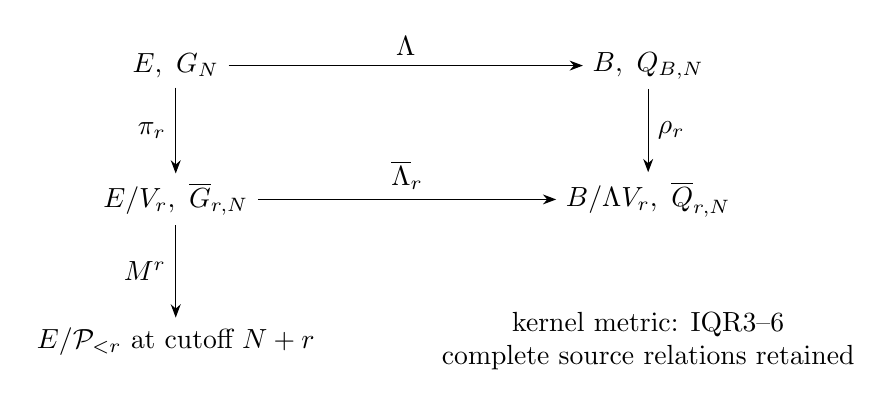
\begin{tikzpicture}[>=Stealth]
\node (e) at (0,2.8) {$E,\ G_N$};
\node (b) at (6,2.8) {$B,\ Q_{B,N}$};
\node (er) at (0,1.1) {$E/V_r,\ \overline G_{r,N}$};
\node (br) at (6,1.1) {$B/\Lambda V_r,\ \overline Q_{r,N}$};
\node (sh) at (0,-.7) {$E/\mathcal P_{<r}$ at cutoff $N+r$};
\draw[->] (e)--node[above]{$\Lambda$}(b);
\draw[->] (e)--node[left]{$\pi_r$}(er);
\draw[->] (b)--node[right]{$\rho_r$}(br);
\draw[->] (er)--node[above]{$\overline\Lambda_r$}(br);
\draw[->] (er)--node[left]{$M^r$}(sh);
\node[align=center] at (6,-.7) {kernel metric: IQR3--6\\
complete source relations retained};
\end{tikzpicture}
\caption{Exact quotient and shifted-source maps. The horizontal
map's degree-zero cohomology is the original kernel. The vertical
source map removes $V_r$; multiplication moves its target to the low
polynomial quotient with the displayed changed cutoff. Every norm is
the attained original norm, not an unweighted coefficient norm.}
\end{figure}

\begin{figure}[ht]\centering
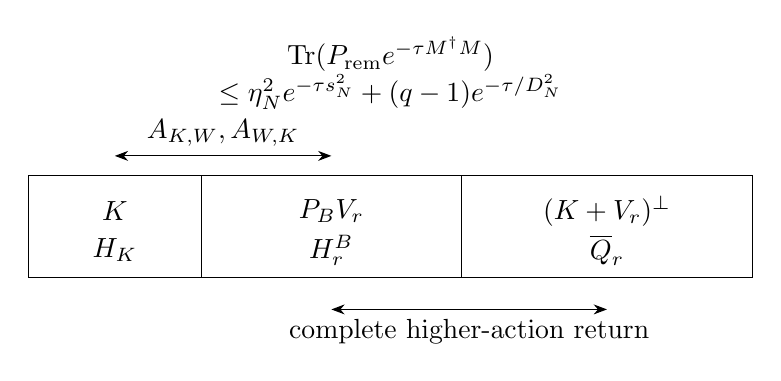
\begin{tikzpicture}[>=Stealth]
\draw (0,0) rectangle (2.2,1.3);
\draw (2.2,0) rectangle (5.5,1.3);
\draw (5.5,0) rectangle (9.2,1.3);
\node at (1.1,.85) {$K$};
\node at (3.85,.85) {$P_BV_r$};
\node at (7.35,.85) {$(K+V_r)^\perp$};
\node at (1.1,.35) {$H_K$};
\node at (3.85,.35) {$H^B_r$};
\node at (7.35,.35) {$\overline Q_r$};
\draw[<->] (1.1,1.55)--node[above]{$A_{K,W},A_{W,K}$}(3.85,1.55);
\draw[<->] (3.85,-.4)--node[below]{complete higher-action return}(7.35,-.4);
\node[align=center] at (4.6,2.6)
 {$\operatorname{Tr}(P_{\rm rem}e^{-\tau M^\dagger M})$\\
 $\le\eta_N^2e^{-\tau s_N^2}+(q-1)e^{-\tau/D_N^2}$};
\end{tikzpicture}
\caption{Exact orthogonal metric blocks, drawn schematically rather
than proportional to dimension. IQR8--10 bounds the residual heat;
IQR21 keeps both complex current cross blocks and the return through
the third block. A positive heat estimate is not used to assign a
complex-current sign.}
\end{figure}

\begin{thebibliography}{9}
\bibitem{IFH} Split-Zero research programme,
\href{https://github.com/KokunoYumeto/zeta-function-research-reader/blob/edd4008690952fb8568a01744e49ad7e180401e9/workbenches/splitzero-tandem/continuations/20260921-original-observation/INVERSE_FLAG_AND_RELATIVE_HEAT.tex}{The original observed inverse-power flag and its relative late heat},
IFH1--21, especially IFH10--21.
\bibitem{IVO} Independent finite derivation,
\href{https://github.com/KokunoYumeto/zeta-function-research-reader/blob/edd4008690952fb8568a01744e49ad7e180401e9/workbenches/splitzero-tandem/continuations/20260921-original-observation/INDEPENDENT_FINITE_OBSERVATION.tex}{IVO1--26, complete finite constants}.
\bibitem{ECL} Split-Zero research programme,
\href{https://github.com/KokunoYumeto/zeta-function-research-reader/blob/5992ad50c0f2a06921f1fcaded7b4e38097c0739/workbenches/splitzero-tandem/continuations/20260920-original-kernel-mixed-determinants/providers/09_INPUT_CUMULATIVE_PROOFS.tex#L28161}{The exact closed equilibrium coefficient, ECL1--17}.
Its full proof is retained in the accompanying cumulative source.
\bibitem{NP} Split-Zero research programme,
\href{https://github.com/KokunoYumeto/zeta-function-research-reader/blob/5992ad50c0f2a06921f1fcaded7b4e38097c0739/workbenches/splitzero-tandem/continuations/20260920-original-kernel-mixed-determinants/providers/09_INPUT_CUMULATIVE_PROOFS.tex#L124542}{NP18--19},
and \href{https://github.com/KokunoYumeto/zeta-function-research-reader/blob/5992ad50c0f2a06921f1fcaded7b4e38097c0739/workbenches/splitzero-tandem/continuations/20260920-original-kernel-mixed-determinants/providers/09_INPUT_CUMULATIVE_PROOFS.tex#L124713}{NP30--31, full proper-source minimum}.
\bibitem{NG} Split-Zero research programme,
\href{https://github.com/KokunoYumeto/zeta-function-research-reader/blob/5992ad50c0f2a06921f1fcaded7b4e38097c0739/workbenches/splitzero-tandem/continuations/20260920-original-kernel-mixed-determinants/providers/NATIVE_GAUSSIAN_TRANSFER.tex#L50}{NG2--3, full original source comparison and multiplication}.
\bibitem{Smallest} Supplied mathematical continuation,
\href{https://github.com/KokunoYumeto/zeta-function-research-reader/blob/0fd693c844aad9117e30ec447c59864a28af10f3/workbenches/splitzero-tandem/continuations/20260921-native-spectral-real-pair/003/NATIVE_SMALLEST_SINGULAR_PROOF.tex}{S1--45}, especially S12--16 and S39--45.
\bibitem{Profile} Supplied mathematical continuation,
\href{https://github.com/KokunoYumeto/zeta-function-research-reader/blob/0fd693c844aad9117e30ec447c59864a28af10f3/workbenches/splitzero-tandem/continuations/20260921-native-spectral-real-pair/003/RETAINED_PROFILE_PROOF.tex}{H1--9, full original outgoing profile}.
\bibitem{Mixed} Supplied mathematical continuation,
\href{https://github.com/KokunoYumeto/zeta-function-research-reader/blob/78ed538f7c00121ab66e9e8adbefc0612c118db8/workbenches/splitzero-tandem/continuations/20260921-mixed-family-proof-source/COMPLETE_MIXED_SOURCE_PROOFS.tex#L129}{Original-metric heat transitions and complete mixed-family control, H17--23},
and \href{https://github.com/KokunoYumeto/zeta-function-research-reader/blob/78ed538f7c00121ab66e9e8adbefc0612c118db8/workbenches/splitzero-tandem/continuations/20260921-mixed-family-proof-source/COMPLETE_MIXED_SOURCE_PROOFS.tex#L528}{C6--10}. The complete original text and TeX accompany this edition.
\bibitem{Stacks} The Stacks Project Authors,
\href{https://stacks.math.columbia.edu/tag/0115}{Tag 0115, acyclic complexes and quasi-isomorphisms};
original author source
\href{https://github.com/stacks/stacks-project/blob/a04446e57ec1fbc252a871afcec7752fb2807b14/homology.tex#L3057}{cochain homotopies}
and \href{https://github.com/stacks/stacks-project/blob/a04446e57ec1fbc252a871afcec7752fb2807b14/homology.tex#L3160}{the definition}.
The finite contraction is supplied explicitly in received equations
(15)--(18); the terminology is not a new general construction.
\bibitem{DLMF} T. H. Koornwinder, R. Wong, R. Koekoek,
R. F. Swarttouw, with W. P. Reinhardt, NIST DLMF Chapter 18,
\href{https://dlmf.nist.gov/18.22.E8}{Meixner--Pollaczek recurrence}
and \href{https://dlmf.nist.gov/18.23.E7}{generating function}.
The original Gamma mass and recurrence in S12--16 retain these
human-source conventions. Their complete specialized estimates
are proved in the cited programme sources.
\end{thebibliography}
\clearpage\part{Independent finite quotient and contraction proofs}
\section{Independent finite derivation of the inverse-quotient identities}\label{independent-finite-derivation-of-the-inverse-quotient-identities}

\subsection{Scope, inputs and reading record}\label{scope-inputs-and-reading-record}

This note verifies equations (3)--(31) of the user-supplied manuscript *The inverse-power theorem gives a quantitative reduction of the original observation complex*. It is an independent finite-dimensional derivation, not a claim to have re-proved the arithmetic inverse-power estimate, the Gamma division estimate, the monic-profile limit, or a Riemann-hypothesis endpoint.

The supplied text is at \nolinkurl{SUPPLIED_INVERSE_SECTOR_REDUCTION.md}. Its equations (3)--(31) were read in full. The preceding programme manuscript *The original observed inverse-power flag and its relative late heat*, \nolinkurl{INVERSE_FLAG_AND_RELATIVE_HEAT.tex}, was read through IFH10 to check the identity of the imported finite comparison. Its public source is \href{https://github.com/KokunoYumeto/zeta-function-research-reader/blob/edd4008690952fb8568a01744e49ad7e180401e9/workbenches/splitzero-tandem/continuations/20260921-original-observation/INVERSE_FLAG_AND_RELATIVE_HEAT.tex}{the complete IFH proof}. The exact source SHA-256 is \nolinkurl{468c92ee4224a3659be44f122efb9fbfc0c2a469624ff5da6d16280aa069a6ca}. In particular IFH1 defines the original observation metric, and IFH2--IFH7 give the finite source/observation sandwich and its passage to attained subquotients. This is programme mathematics, not an original human primary paper. No external primary-source theorem is silently attributed to it.

The mathematical task received from the root was to derive the Schur, quotient, chain-homotopy, inverse-division and observed-feedback identities, preserving the original objects and identifying any exact correction with a proof. Root retains source tracing and all later equations. No owner source, remote repository, or publication was changed by this task.

\subsection{1. Original finite objects and the minimum formula}\label{original-finite-objects-and-the-minimum-formula}

All adjoints denoted by a star in coordinate formulas are conjugate transposes. A metric matrix records a Hermitian form, not a replacement of the original form by the identity.

Let the full original polynomial be monic of degree q with Q(0) nonzero. The algebra is E=C{[}y{]}/(Q), represented in the complete ordered basis 1,y,\ldots,y\^{}(q−1). Multiplication by y is the invertible operator M. Let G be the specified positive Hermitian metric on E, let Λ:E→B be onto, and let I\_K:C\^{}m→E be the fixed full-column frame of K=ker Λ. Set

\[
H_K=I_K^*GI_K,\qquad
Q_B=(\Lambda G^{-1}\Lambda^*)^{-1},\qquad
L_B=G^{-1}\Lambda^*Q_B.
\]

For every onto matrix A from a space with metric H, the unique least-norm solution of Ax=b is

\[
S_Ab=H^{-1}A^*(AH^{-1}A^*)^{-1}b.
\]

Indeed \(AS_A=I\), and for \(z\in\ker A\), \(z^*HS_Ab=z^*A^*(AH^{-1}A^*)^{-1}b=0\). Every solution is \(S_Ab+z\); its squared norm is \(b^*(AH^{-1}A^*)^{-1}b+z^*Hz\). This proves attainment, uniqueness, the quotient metric, and the fact that S\_A is an isometry from that quotient metric. It also proves A is a contraction and that S\_AA is the original-metric orthogonal projection onto (ker A)\^{}⊥.

Apply this to Λ. Then P\_B=L\_BΛ is the original G-orthogonal projection onto K\^{}⊥. The complementary projection is

\[
P_K=I_KH_K^{-1}I_K^*G,\qquad P_B+P_K=I_E.
\]

For 0≤r≤q, retain the ordered inverse-power map

\[
U_rd=\sum_{j=1}^r d_j[y^{-j}],\qquad V_r=\operatorname{im}U_r.
\]

It is injective: multiplying U\_rd=0 by M\^{}r yields \(\sum_{j=1}^rd_jy^{r-j}=0\) in E, and the representative has degree less than q. Thus all its coefficients vanish. In the observation sector under consideration the imported IP lower factor is positive, so Φ\_r=ΛU\_r is also injective. Equivalently K∩V\_r=0. Define

\[
H^E=U_r^*GU_r,\quad H^B=\Phi_r^*Q_B\Phi_r,\quad
\Gamma=I_K^*GU_r.
\]

The finite input used below is precisely \(aH^E\preceq H^B\preceq H^E\), with a\textgreater0. Because H\^{}E is positive, this also entails a≤1. The stated arithmetic IP theorem supplies a and its lower bound exp(−ε); this finite derivation does not change that input.

\subsection{2. The two Schur complements, their eigenvalues and their exact loss}\label{the-two-schur-complements-their-eigenvalues-and-their-exact-loss}

Since P\_B is G-self-adjoint and idempotent,

\[
H^B=U_r^*GP_BU_r
=H^E-U_r^*GP_KU_r
=H^E-\Gamma^*H_K^{-1}\Gamma. \tag{F3}
\]

For \(z\in\mathbb C^m\) the quotient norm of I\_Kz modulo V\_r is the attained minimum of \((I_Kz+U_rd)^*G(I_Kz+U_rd)\) over all d.~Completing the exact quadratic form yields the minimizing coefficient \(d=-(H^E)^{-1}\Gamma^*z\) and hence

\[
\widehat H_K=H_K-\Gamma(H^E)^{-1}\Gamma^*. \tag{F4}
\]

This minimum remains positive because K∩V\_r=0. The minimum representative is \((I-P_V)I_Kz\), where \(P_V=U_r(H^E)^{-1}U_r^*G\) is the original orthogonal projection onto V\_r.

For the finite spectral comparison define, without altering either physical metric,

\[
T=H_K^{-1/2}\Gamma(H^E)^{-1/2}.
\]

The original metric matrices factor exactly as

\[
H^B=(H^E)^{1/2}(I_r-T^*T)(H^E)^{1/2},\qquad
\widehat H_K=H_K^{1/2}(I_m-TT^*)H_K^{1/2}.
\]

The positive eigenvalues of T*T and TT* coincide, with multiplicity: if \(T^*Tv=\mu v\) and \(\mu>0\), then \(Tv\ne0\) and \(TT^*(Tv)=\mu Tv\); the inverse correspondence on this eigenspace is \(\mu^{-1}T^*\). Their number is \(\nu=\operatorname{rank}T=\operatorname{rank}\Gamma\). The remaining eigenvalues are zero. IP gives \(0\preceq T^*T\preceq(1-a)I_r\), so the same nonzero-eigenvalue calculation gives \(0\preceq TT^*\preceq(1-a)I_m\). Consequently

\[
aH_K\preceq\widehat H_K\preceq H_K. \tag{F5}
\]

One can obtain the determinant equality without a spectral argument by taking the determinant of the same block Gram \(\begin{psmallmatrix}H_K&\Gamma\\\Gamma^*&H^E\end{psmallmatrix}\) in its two block orders. The equality is

\[
\det H_K\det H^B=\det H^E\det\widehat H_K,
\quad
\delta:=\log\frac{\det H^E}{\det H^B}
=\log\frac{\det H_K}{\det\widehat H_K}
=-\log\det(I_r-T^*T). \tag{F6}
\]

If the ν nonzero eigenvalues of T*T are μ\_j, then \(\delta=-\sum_{j=1}^{\nu}\log(1-\mu_j)\). Every factor 1−μ\_j lies in {[}a,1{]}. Thus

\[
0\le\delta\le\nu\log(1/a)\le\min(m,r)\varepsilon
\quad\text{when }a\ge e^{-\varepsilon}. \tag{F7}
\]

This proves the precise rank loss in (7), not a loss counted r times when r\textgreater m. With the manuscript's stated uniform ε=o(q) and m=O(k), it implies δ=o(kq) exactly as in (8). This is a propagation of the stated input, not a separate verification of its arithmetic range.

For the four-cutoff signs +,+,−,−, all four losses lie in the same interval {[}0,d{]}, where d=min(m,r)ε. Their signed sum belongs to {[}−2d,2d{]}: the sum of the two positively signed losses and the sum of the two negatively signed losses each belong to {[}0,2d{]}. Since log det Hhat=log det H\_K−δ, this proves the factor two in (9). No cancellation beyond the common nonnegative interval has been assumed.

\subsection{3. Explicit quotient coordinates and their attained metric}\label{explicit-quotient-coordinates-and-their-attained-metric}

Let rem\_Q denote the full degree-below-q representative. Define

\[
\pi_r[p]=\mathscr D^r(\operatorname{rem}_Q(y^rp)),\qquad
\mathscr D^rf=(f-\operatorname{Tay}_{<r}f)/y^r.
\tag{F10}
\]

This is well-defined on E, because replacing p by p+Qa does not change rem\_Q(y\^{}rp). It maps into P\_\textless q−r. Its kernel consists exactly of classes whose M\^{}r-image is in P\_\textless r. Since M\^{}rV\_r=P\_\textless r, invertibility of M\^{}r gives ker π\_r=V\_r. Let ι\_r be the ordinary degree-below-(q−r) inclusion. For p in this coefficient space, y\^{}rp has degree below q and its first r coefficients vanish; hence π\_rι\_rp=p.~Thus π\_r is onto.

The general minimum calculation in Section 1 yields

\[
\overline G_r=(\pi_rG^{-1}\pi_r^*)^{-1},\qquad
S_r=G^{-1}\pi_r^*\overline G_r. \tag{F11}
\]

Here S\_r is the minimum section, and S\_rπ\_r=I−P\_V. The quotient coordinate metric is therefore the attained one, not the raw polynomial Gram. Direct substitution gives

\[
(\pi_rI_K)^*\overline G_r(\pi_rI_K)
=I_K^*G(I-P_V)I_K=\widehat H_K.
\]

The physical substitution \(S=c+iy\) is retained by its full triangular map \[
(T_c)_{ab}=\binom ba c^{b-a}i^a\quad(a\le b),\qquad (T_c)_{ab}=0\quad(a>b).
\] It sends \(S\)-coefficients to \(y\)-coefficients. Therefore \(I_K^y=T_cI_K^S\) and \(G^S=T_c^*G^yT_c\), and both sides give the same fixed-kernel Gram. The diagonal phases \(i^a\) are retained.

\subsection{4. The quotient observation, its metric and the chain contraction}\label{the-quotient-observation-its-metric-and-the-chain-contraction}

Because Φ\_r is injective, choose r rows I with invertible minor Φ\_I, and let J be the remaining row indices. With coordinate selectors R\_I and R\_J, define the fixed algebraic quotient matrix

\[
\rho_r=R_J-\Phi_J\Phi_I^{-1}R_I.
\]

It kills Φ\_r. Its restriction to the coordinate complement supported on J is the identity, so it is onto and has kernel W\_r=im Φ\_r. This formula depends on the original algebraic maps, not on the cutoff metric. Define

\[
\overline\Lambda_r=\rho_r\Lambda\iota_r.
\]

Since x−ι\_rπ\_rx lies in V\_r and ρ\_rΛ kills V\_r, barΛ\_rπ\_r=ρ\_rΛ. Onto-ness follows from that of ρ\_rΛ. If barΛ\_rπ\_rx=0, then Λx=Λv for some v∈V\_r, so x−v∈K and π\_rx∈π\_rK. Conversely π\_rK is killed. The restriction π\_r:K→ker barΛ\_r is injective and onto. This proves all arrows and exactness in (12)--(13).

For the target quotient the attained metric is

\[
\overline Q_r=(\rho_rQ_B^{-1}\rho_r^*)^{-1}.
\]

The inverse of this matrix is exactly \[
\begin{aligned}
\rho_r\Lambda G^{-1}\Lambda^*\rho_r^*
&=\overline\Lambda_r\pi_rG^{-1}\pi_r^*\overline\Lambda_r^*\\
&=\overline\Lambda_r\,\overline G_r^{-1}\overline\Lambda_r^* .
\end{aligned}
\] Inverting proves (14) and equality of the two orders of complete minimum, without identifying either quotient metric with a raw coefficient Gram.

Now set

\[
h=U_r(H^B)^{-1}\Phi_r^*Q_B:B\longrightarrow E. \tag{F15}
\]

Then hΦ\_r=U\_r, so hΛ is idempotent with image V\_r. Its kernel is the preimage under Λ of the Q\_B-orthogonal complement to W\_r. Meanwhile \(P_W=\Lambda h=\Phi_r(H^B)^{-1}\Phi_r^*Q_B\) is the original Q\_B-orthogonal projection onto W\_r. The degree-zero projection hΛ need not be orthogonal.

Write hb=U\_rd. The equality d=(H\^{}B)\^{}(−1)Φ\_r*Q\_Bb gives

\[
\|hb\|_G^2=d^*H^Ed\le a^{-1}d^*H^Bd
=a^{-1}\|P_Wb\|_{Q_B}^2\le a^{-1}\|b\|_{Q_B}^2.
\]

Thus \(\|h\|\le a^{-1/2}\), proving (16) with its exact metric domains.

Let \(S_\rho=Q_B^{-1}\rho_r^*\overline Q_r\) be the minimum section of ρ\_r. Since S\_ρρ\_r=I−P\_W, the fully explicit chain section of p=(π\_r,ρ\_r) is

\[
j^0=(I_E-h\Lambda)S_r,
\qquad j^1=S_\rho. \tag{F17a}
\]

First π\_rj\^{}0=π\_rS\_r=I and ρ\_rj\^{}1=I. Secondly,

\[
\Lambda j^0=(I_B-\Lambda h)\Lambda S_r
=S_\rho\rho_r\Lambda S_r
=S_\rho\overline\Lambda_r=j^1\overline\Lambda_r.
\]

Thus j is a chain map. The difference x−S\_rπ\_rx belongs to V\_r and I−hΛ kills V\_r; hence j\^{}0π\_r=I−hΛ. The other degree gives j\^{}1ρ\_r=I−Λh. Regard h:B→E as a degree −1 map, with its other component zero. For the differential d=Λ these two equalities are exactly

\[
I-jp=dh+hd. \tag{F17b}
\]

This proves the finite chain-homotopy equivalence (18). It fixes K pointwise: for x∈K, j\^{}0π\_rx=(I−hΛ)x=x. No infinite theta complex is introduced by this calculation.

\subsubsection{Complete polynomial relation spaces remain present}\label{complete-polynomial-relation-spaces-remain-present}

Let the actual source P\_N have its positive source metric, and let J\_N:P\_N→E be the full remainder map, with minimum section L\_N. Then J\_NL\_N=I and L\_N is an isometry from G. The lifted homotopy \(\widetilde h=L_Nh\) has exactly the same norm. Its range is L\_NV\_r. Moreover \(\widetilde h\Lambda J_N\) vanishes on the complete original relation space \(\ker J_N=Q\mathcal P_{N-q}\), and this relation space is orthogonal to L\_NE and therefore to L\_NV\_r.

There is a corresponding reduction of {[}P\_N→B{]} by the contractible subcomplex {[}L\_NV\_r→W\_r{]}. Its source quotient is P\_N/(L\_NV\_r), not an identification of P\_N with E: every original Q-relation remains in degree-zero cohomology. The same proof with differential ΛJ\_N and homotopy L\_Nh gives the contraction. This specifies exactly what the manuscript's polynomial-source lift preserves.

\subsection{5. Exact determinant allocation and its fixed frame factor}\label{exact-determinant-allocation-and-its-fixed-frame-factor}

The Gram of the augmented kernel K+V\_r in the fixed ordered frame {[}I\_K,U\_r{]} has blocks H\_K,Γ,Γ*,H\^{}E. Its determinant is

\[
\det([I_K,U_r]^*G[I_K,U_r])=\det H_K\det H^B. \tag{F19}
\]

Choose any fixed right inverse Z of ρ\_r and set C={[}Φ\_r,Z{]}. This square matrix is invertible. In that frame the Q\_B Gram has leading block H\^{}B and lower Schur complement barQ\_r. Therefore the complete equality is

\[
|\det C|^2\det Q_B=\det H^B\det\overline Q_r,
\]

or

\[
\log\det\overline Q_r
=\log\det Q_B-\log\det H^B+2\log|\det C|. \tag{F20}
\]

C is fixed across the four cutoffs, so the last term cancels under their signs. This is precisely (20), including the coefficient-frame constant before the return is taken. Combined with (F19), the signs of the two redistributed terms in (21) are + and −. Any use of the evaluated coefficient Cfrak belongs to the imported IFH coefficient theorem; the allocation itself has no asymptotic error.

\subsection{6. Inverse multiplication as exact Taylor division between quotients}\label{inverse-multiplication-as-exact-taylor-division-between-quotients}

For x∈E retain its actual minimum source representative L\_Nx, and write

\[
L_Nx=\sum_{j=0}^{s-1}c_j(x)y^j+y^s\mathscr D^sL_Nx.
\]

Apply J\_N, and then multiply by M\^{}(−s). The result is

\[
M^{-s}x=J_N\mathscr D^sL_Nx+
\sum_{n=1}^sc_{s-n}(x)[y^{-n}]. \tag{F22}
\]

Thus the ordering in F\_(s,N) is exactly (F\_(s,N)x)\emph{n=c}(s−n)(x), as in (22). No assertion has been made that polynomial Taylor coefficients themselves are well-defined on E; the map L\_N supplies their specific representative.

For the norm in (23), the supplied Gamma comparison has the form ell\_(k,N) H\_Gamma≤H\_native on degrees ≤N and H\_native≤u\_k H\_Gamma on the output range. Apply these two comparisons on the outside of the s-fold division estimate, giving

\[
\|\mathscr D^sf\|_{\rm native}
\le \sqrt{u_k}\|\mathscr D^sf\|_\Gamma
\le\sqrt{u_k}(a_N^\Gamma)^s\|f\|_\Gamma
\le\sqrt{u_k/\ell_{k,N}}(a_N^\Gamma)^s\|f\|_{\rm native}.
\]

The source minimum L\_N is an isometry and J\_N is a contraction, so \textbar\textbar J\_N D\^{}s L\_N\textbar\textbar≤B\_(s,N). Only one comparison ratio occurs. This derives the use of the imported division bound, not its original Gamma proof.

Since \(M^{-s}V_r\subset V_{r+s}\), the map

\[
\mathcal I_{r,s}=\pi_{r+s}M^{-s}\iota_r:E/V_r\to E/V_{r+s}
\]

is well-defined for r+s≤q. For the canonical coordinate p of degree below q−r, calculate

\[
\pi_{r+s}M^{-s}\iota_rp
=\mathscr D^{r+s}\operatorname{rem}_Q(M^{r+s}M^{-s}p)
=\mathscr D^{r+s}(y^rp)=\mathscr D^sp. \tag{F24}
\]

The second equality means the representative of the algebraic product: \(M^{r+s}M^{-s}p=M^rp\), whose representative is y\^{}rp since its degree is below q. Hence the kernel is exactly P\_\textless s inside P\_\textless q−r and the map is onto P\_\textless q−r−s. Equivalently, \(M^sV_{r+s}=V_r\oplus\mathcal P_{<s}\): multiplying by M\^{}r sends these two summands to P\_\textless r and \(\operatorname{span}(y^r,\ldots,y^{r+s-1})\), disjoint complete monomial ranges of degree below q. This proves (25), including its first injection.

For the norm, take the actual minimum representative x=S\_rz of a quotient class z. The last term of (F22) belongs to V\_s⊂V\_(r+s), so

\[
\mathcal I_{r,s}z=\pi_{r+s}J_N\mathscr D^sL_NS_rz.
\]

Each outer quotient map is a contraction and S\_r an isometry in the attained metrics. This gives (26). Directly from \(M^{-t}M^{-s}=M^{-s-t}\), or from \(\mathscr D^t\mathscr D^s=\mathscr D^{s+t}\), one obtains (27) with its degree-changing domain and codomain. No fixed quotient is being treated as M-invariant.

\subsection{7. Complete observed leakage and composition memory}\label{complete-observed-leakage-and-composition-memory}

Let barL\_r be the attained minimum section of barΛ\_r and let barP\^{}K\_r=I−barL\_r barΛ\_r. It is the original quotient-metric orthogonal projection onto ker barΛ\_r. The observed map is

\[
\mathcal B_{r,s}=\overline\Lambda_{r+s}
\mathcal I_{r,s}\overline L_r.
\]

The section is an isometry and barΛ\_(r+s) is a contraction. Consequently \textbar\textbar B\_(r,s)\textbar\textbar≤B\_(s,N), exactly (28). Insert I=barL\_r barΛ\_r+barP\^{}K\_r to obtain

\[
\overline\Lambda_{r+s}\mathcal I_{r,s}
=\mathcal B_{r,s}\overline\Lambda_r
+\overline\Lambda_{r+s}\mathcal I_{r,s}\overline P^K_r. \tag{F29}
\]

All three factors in the last term have norm ≤1, B\_(s,N), ≤1 in their actual metrics, proving the same leakage bound.

For the composition use the exact identity (27) and subtract the observed product. The middle difference is \(I-\overline L_{r+s}\overline\Lambda_{r+s}=\overline P^K_{r+s}\), so

\[
\begin{aligned}
\mathcal B_{r,s+t}-\mathcal B_{r+s,t}\mathcal B_{r,s}
={}&\overline\Lambda_{r+s+t}\mathcal I_{r+s,t}
\overline P^K_{r+s}\mathcal I_{r,s}\overline L_r.
\end{aligned}\tag{F30}
\]

The sign is positive. The norm is at most B\_(t,N)B\_(s,N). On the retained injective conductor domain ker barΛ\_(r+s)=π\_(r+s)K has dimension m, and the rank is therefore at most m. Even outside injectivity of a particular inverse sector, the kernel dimension is at most m because its kernel remains π\_(r+s)K; the formulas involving its quotient metric still use its actual target quotient dimension.

Finally ρ\_(r+s)ΛU\_s=0 since ΛV\_s⊂W\_(r+s). Apply ρ\_(r+s)Λ to (F22) and restrict the input by I\_K. This proves

\[
\rho_{r+s}\Lambda M^{-s}I_K
=\rho_{r+s}\Lambda J_N\mathscr D^sL_NI_K. \tag{F31}
\]

The frame I\_K is an isometry from its retained coordinate metric H\_K to its physical image, and ρ\_(r+s)Λ is a contraction for the attained target metric. This proves the stated norm bound, without quotienting or changing the metric on the original K.

\subsection{8. Exact finite verification and conclusion}\label{exact-finite-verification-and-conclusion}

The companion \texttt{verify\_exact.py} uses SymPy exact rational complex arithmetic, the full polynomial \(Q=y^6+2y^4-y^3+3y+2\), an eight-dimensional positive source Gram with nonzero imaginary off-diagonal entries, its original quotient Gram, and a fixed onto observation and fixed two-dimensional kernel frame. The source metric is constructed explicitly, then G and all sections are obtained by their stated attained-minimum formulas. No floating or identity-metric replacement is used.

The script checks r=1,2,3, full Schur complements, all quotient and chain maps, both homotopy identities, the exact frame determinant factor, inverse Taylor decomposition, and the observed feedback identity. It requires the observed composition defect to be nonzero, so success cannot result merely from accidentally selecting an invariant observed sector. The actual result count and script hash are in \nolinkurl{EXACT_CHECKS.json}.

No correction to the finite identities (3)--(31) was found. The two details made explicit here are already consistent with the supplied manuscript: (i) the fixed frame factor 2 log\textbar det C\textbar{} in (F20) exists before the four-cutoff return; (ii) the polynomial-source contraction quotients by L\_NV\_r and retains its entire Q-relation kernel, rather than replacing that larger source complex by {[}E→B{]}.

\clearpage\part{Independent covariance-angle derivation}
\section{Independent covariance-angle derivation}\label{independent-covariance-angle-derivation}

Date: 21 September 2026.

This file checks IQR15--19 and the algebra of IQR2 in \nolinkurl{INVERSE_QUOTIENT_RECEIVERS.tex}. It proves the finite matrix statements independently, retains the original metric and the complete source covariance, and spells out the four-cutoff estimate. It does not change the mathematical period domain or assert a new analytic estimate for the source covariance.

The exact finite angle estimate is correct. A stronger estimate using the individual covariance eigenvalues is proved below. The coefficient identity is correct when the retained endpoint value \(\psi(0)=\log(4/\pi)\) is included explicitly. No determinant factor is missing when the frame on \(K+V\) is the stated concatenation.

\subsection{Reading and derivation record}\label{reading-and-derivation-record}

The source inspected for this derivation was \nolinkurl{INVERSE_QUOTIENT_RECEIVERS.tex}, SHA-256 \nolinkurl{42664D36E612DEB49550850DCAA15EF2774B58682A07CDF7F707DF5F3D3F9BA2}. The whole file was read; the independent calculations below concern IQR2 and IQR13--19, together with the exact Schur identity used in IQR3. The separate endpoint definition was checked in \nolinkurl{../publication_003/NATIVE_SMALLEST_SINGULAR_PROOF.tex}, S2--S3, lines 31--41, SHA-256 \nolinkurl{C7DD360325DC475B82CABBC65F2DC01D5C67711B85951A1837CD3E7F52415BBB}. That reading was bounded to its opening theorem and definitions, lines 1--58. Its public source locator is \href{https://github.com/KokunoYumeto/zeta-function-research-reader/blob/0fd693c844aad9117e30ec447c59864a28af10f3/workbenches/splitzero-tandem/continuations/20260921-native-spectral-real-pair/003/NATIVE_SMALLEST_SINGULAR_PROOF.tex\#L31}{S2--S3 in the retained smallest-singular proof}. This file is a new finite-dimensional derivation, not a transcription of that source.

The proof is complete for the stated finite hypotheses. The asymptotic application uses the already stated IQR1 size estimate and the explicitly displayed covariance-size hypotheses; those earlier analytic results are not independently rederived here.

\subsection{1. Exact objects, frames, and covariance}\label{exact-objects-frames-and-covariance}

Let \(E=\mathbb C^n\) in its fixed coefficient coordinates. Let \(G_0\) be a positive-definite Hermitian matrix, and let \(\Omega\) be a positive-semidefinite Hermitian matrix. For every real \(t\ge0\), set

\[
G(t)=(G_0^{-1}+t\Omega)^{-1}.
\tag{CA1}
\]

Every inverse in CA1 exists: for \(x\ne0\), \(x^*(G_0^{-1}+t\Omega)x\ge x^*G_0^{-1}x>0\). Use the inner product \(\langle x,y\rangle_t=x^*G(t)y\), with conjugate linearity in the first argument.

Keep fixed subspaces \(K,V\subset E\), with \(K\cap V=\{0\}\), dimensions \(m,r\), and fixed full column frames \(I_K:\mathbb C^m\to E\), \(U:\mathbb C^r\to E\). Set \(S_0=K+V\), and use precisely the concatenated frame \(I_{S_0}=[I_K,U]\). Thus \(\dim S_0=m+r\le n\). For \(X=K,V,S_0\), write

\[
H_X(t)=I_X^*G(t)I_X,
\qquad
\Gamma(t)=I_K^*G(t)U.
\tag{CA2}
\]

Here \(I_V=U\). All three Gram matrices are positive definite because their frames are injective. Define

\[
\delta(t)=\log\det H_K(t)+\log\det H_V(t)
-\log\det H_{S_0}(t).
\tag{CA3}
\]

The logarithms are the real logarithms of positive determinants. If one subspace has dimension zero, its determinant is 1 and \(\delta\equiv0\); every assertion below then holds with a zero right side.

For the source in IQR13, the matrix in CA1 is the full matrix

\[
\Omega=F_ZH_Z^+F_Z^*,
\qquad H_Z\succeq0,
\qquad \ker H_Z\subseteq\ker F_Z.
\tag{CA4}
\]

Indeed \(\Omega=BB^*\) with \(B=F_Z(H_Z^+)^{1/2}\), so \(\Omega\succeq0\). If \(\Pi\) is the Euclidean projection onto \(\operatorname{ran}H_Z\), the kernel hypothesis gives \(F_Z=F_Z\Pi\). The matrix \((H_Z^+)^{1/2}\) is invertible on \(\operatorname{ran}H_Z\), so \(\operatorname{rank}\Omega=\operatorname{rank}B=\operatorname{rank}F_Z\). Neither this factorization nor anything below removes a cross term of \(H_Z\), \(H_Z^+\), or \(\Omega\).

\subsection{2. The Schur identity and exact quotient meaning}\label{the-schur-identity-and-exact-quotient-meaning}

In the stated concatenated frame,

\[
H_{S_0}(t)=
\begin{pmatrix}H_K(t)&\Gamma(t)\\
\Gamma(t)^*&H_V(t)\end{pmatrix}.
\tag{CA5}
\]

Suppress \(t\) within this section. Left multiplication by \(\begin{psmallmatrix}I&0\\-\Gamma^*H_K^{-1}&I\end{psmallmatrix}\) is determinant preserving and gives an upper block triangular matrix. Consequently

\[
\det H_{S_0}
=\det H_K\det(H_V-\Gamma^*H_K^{-1}\Gamma).
\tag{CA6}
\]

Eliminating the other off-diagonal block gives

\[
\det H_{S_0}
=\det H_V\det(H_K-\Gamma H_V^{-1}\Gamma^*).
\tag{CA7}
\]

Both Schur complements are positive definite. For example, for \(a\ne0\), insert \((a,-H_V^{-1}\Gamma^*a)\ne0\) into the positive quadratic form CA5 to obtain \(a^*(H_K-\Gamma H_V^{-1}\Gamma^*)a>0\).

Let \(\pi:E\to E/V\) be represented by any fixed onto matrix whose kernel is \(V\). Its attained quotient metric is

\[
\overline G(t)=(\pi G(t)^{-1}\pi^*)^{-1}.
\tag{CA8}
\]

To verify this formula directly, for a quotient coordinate \(b\), put \(x_*=G(t)^{-1}\pi^*\overline G(t)b\). Then \(\pi x_*=b\), and for every \(v\in\ker\pi\), \(v^*G(t)x_*=v^*\pi^*\overline G(t)b=0\). Every other lift equals \(x_*+v\), whose squared norm is \(x_*^*G(t)x_*+v^*G(t)v\). Hence \(x_*\) is the unique minimum lift and the attained squared norm is \(b^*\overline G(t)b\).

For the quotient image of \(I_Ka\), all lifts have the form \(I_Ka+Uz\). Their squared norms equal

\[
a^*H_Ka+a^*\Gamma z+z^*\Gamma^*a+z^*H_Vz.
\]

Completion of this quadratic form gives the unique minimizer \(z=-H_V^{-1}\Gamma^*a\). Therefore the quotient kernel Gram is exactly

\[
\widehat H_K(t)
=(\pi I_K)^*\overline G(t)(\pi I_K)
=H_K(t)-\Gamma(t)H_V(t)^{-1}\Gamma(t)^*.
\tag{CA9}
\]

The disjointness hypothesis makes \(\pi I_K\) injective. Equations CA3 and CA7 give

\[
\delta(t)=\log\det H_K(t)-\log\det\widehat H_K(t).
\tag{CA10}
\]

For the original observation \(\Lambda:E\to B\) with \(\ker\Lambda=K\), the identical minimum calculation gives \(H_V^B(t)=H_V(t)-\Gamma(t)^*H_K(t)^{-1}\Gamma(t)\), using the attained metric \((\Lambda G(t)^{-1}\Lambda^*)^{-1}\) on \(B\). Thus

\[
\delta(t)=\log\det H_V(t)-\log\det H_V^B(t).
\tag{CA11}
\]

This proves the exact morphism between the two angle losses. It retains the physical subspaces and all cross-Gram entries.

For an explicit expression, define

\[
B_t=H_K(t)^{-1/2}\Gamma(t)H_V(t)^{-1/2}.
\]

From CA6,

\[
\delta(t)=-\log\det(I_r-B_t^*B_t)
=-\sum_{j=1}^{\min(m,r)}\log(1-c_j(t)^2)\ge0,
\tag{CA12}
\]

where the \(c_j(t)\) are the singular values of \(B_t\), including zeros. Positivity of the Schur complement proves \(c_j(t)<1\).

There is no unstated frame constant in these equations. Replacing \(I_K,U\) by \(I_KT_K,UT_V\), with both matrices invertible, changes the three log determinants in CA3 by \(2\log|\det T_K|\), \(2\log|\det T_V|\), and their sum. These changes cancel. If instead a separate frame \(I_{S_0}T\) is used on \(S_0\) while the first two frames are retained, CA3 acquires the constant \(-2\log|\det T|\). Its nonnegativity need not survive, although the change \(\delta(t)-\delta(0)\) is unchanged for fixed \(T\). This is why the concatenation in IQR15 matters for IQR18.

\subsection{3. Exact differentiated identity}\label{exact-differentiated-identity}

Differentiating \((G_0^{-1}+t\Omega)G(t)=I\) gives

\[
G'(t)=-G(t)\Omega G(t).
\tag{CA13}
\]

For a fixed full frame \(I_X\), the determinant differential follows from the cofactor identity for the determinant:

\[
\frac{d}{dt}\log\det H_X(t)
=\operatorname{Tr}(H_X(t)^{-1}I_X^*G'(t)I_X).
\]

Define the original-metric projection and its exact Euclidean transform by

\[
P_X(t)=I_XH_X(t)^{-1}I_X^*G(t),
\qquad
\widetilde P_X(t)=G(t)^{1/2}P_X(t)G(t)^{-1/2}.
\tag{CA14}
\]

The first operator is idempotent, fixes \(X\), and satisfies \(G(t)P_X(t)=P_X(t)^*G(t)\). The second is \(G(t)^{1/2}I_XH_X(t)^{-1}I_X^*G(t)^{1/2}\), so it is the Euclidean orthogonal projection onto the actual transformed subspace \(G(t)^{1/2}X\).

Substitution of CA13 and cyclicity of the finite trace give

\[
\frac{d}{dt}\log\det H_X(t)
=-\operatorname{Tr}\bigl(G(t)^{1/2}\Omega G(t)^{1/2}
\widetilde P_X(t)\bigr).
\tag{CA15}
\]

Consequently, for \(t>0\),

\[
t\delta'(t)=-\operatorname{Tr}(D_tA_t),
\quad D_t=tG(t)^{1/2}\Omega G(t)^{1/2},
\quad A_t=\widetilde P_K(t)+\widetilde P_V(t)-\widetilde P_{S_0}(t).
\tag{CA16}
\]

This proves IQR15. It differentiates the original fixed-frame Gram matrices. No derivative of a moving transformed frame has been omitted: the transformed projections occur only after evaluating that derivative by CA15.

\subsection{4. Complete spectrum of the projection-pair operator}\label{complete-spectrum-of-the-projection-pair-operator}

Fix \(t\), and write \(\mathcal K=G(t)^{1/2}K\), \(\mathcal V=G(t)^{1/2}V\). Their intersection remains zero because \(G(t)^{1/2}\) is invertible. The matrices

\[
T_K=G(t)^{1/2}I_KH_K(t)^{-1/2},
\qquad T_V=G(t)^{1/2}UH_V(t)^{-1/2}
\]

have orthonormal columns, and \(T_K^*T_V=B_t\). Choose a singular-value decomposition of \(B_t\), rotating these two orthonormal frames accordingly. If \(p=\min(m,r)\), the resulting unit vectors satisfy

\[
e_i^*e_j=\delta_{ij},\qquad f_i^*f_j=\delta_{ij},
\qquad e_i^*f_j=c_i\delta_{ij},
\tag{CA17}
\]

for paired indices, with all additional cross products zero. Here \(e_i\in\mathcal K\) and \(f_i\in\mathcal V\), not the untransformed physical subspaces. By Cauchy--Schwarz, \(c_i\le1\). Equality would give \(f_i=e_i\), contradicting \(\mathcal K\cap\mathcal V=0\). Thus \(0\le c_i<1\), agreeing with CA12.

For each paired index put \(h_i=(f_i-c_ie_i)/\sqrt{1-c_i^2}\). Equations CA17 show that all pairs \((e_i,h_i)\) are orthonormal and mutually orthogonal. The extra unpaired vectors are orthogonal to their sum. On the pair \((e_i,h_i)\), the two projections are

\[
\widetilde P_K=\begin{pmatrix}1&0\\0&0\end{pmatrix},
\qquad
\widetilde P_V=\begin{pmatrix}c_i^2&c_i\sqrt{1-c_i^2}\\
c_i\sqrt{1-c_i^2}&1-c_i^2\end{pmatrix}.
\]

The projection onto \(\mathcal K+\mathcal V\) is the identity on that pair. Hence

\[
A_t\big|_{\operatorname{span}(e_i,h_i)}
=\begin{pmatrix}c_i^2&c_i\sqrt{1-c_i^2}\\
c_i\sqrt{1-c_i^2}&-c_i^2\end{pmatrix},
\qquad \det(\lambda I-A_t)=\lambda^2-c_i^2.
\tag{CA18}
\]

The eigenvalues on this pair are \(+c_i,-c_i\). If \(c_i=0\), the entire block is zero. An unpaired vector lies in one subspace and is orthogonal to the other, so \(A_t\) is zero on it as well. Outside \(\mathcal K+\mathcal V\), all three projections vanish. This accounts for every dimension of \(E\).

Thus the nonzero eigenvalues of \(A_t\) are exactly \(\nu(t)\) pairs \(+c_i,-c_i\), where

\[
\nu(t)=\operatorname{rank}B_t
=\operatorname{rank}(I_K^*G(t)U)\le\min(m,r).
\tag{CA19}
\]

In particular, if \(A_t=A_{t,+}-A_{t,-}\) is its positive/negative spectral decomposition, then

\[
0\preceq A_{t,+},A_{t,-}\preceq I,
\qquad
\operatorname{rank}A_{t,+}=\operatorname{rank}A_{t,-}=\nu(t).
\tag{CA20}
\]

This proves the complete IQR16 spectrum, including the orthogonal and exterior directions.

\subsection{5. Covariance spectrum and the sharp rank-dependent trace estimate}\label{covariance-spectrum-and-the-sharp-rank-dependent-trace-estimate}

Set

\[
C=G_0^{1/2}\Omega G_0^{1/2},\qquad
d=\operatorname{rank}\Omega=\operatorname{rank}C,
\qquad c=\|C\|.
\tag{CA21}
\]

Write the eigenvalues of \(C\) in decreasing order as \(\lambda_1\ge\cdots\ge\lambda_n\ge0\). Direct multiplication proves

\[
G(t)=G_0^{1/2}(I+tC)^{-1}G_0^{1/2},
\quad
G_0^{-1/2}G(t)\Omega G_0^{1/2}=(I+tC)^{-1}C.
\tag{CA22}
\]

Also \(G(t)^{-1/2}(tG(t)\Omega)G(t)^{1/2}=D_t\). Therefore the positive matrix \(D_t\) has the exact ordered eigenvalues

\[
\mu_j(t)=\frac{t\lambda_j}{1+t\lambda_j},
\qquad
\operatorname{rank}D_t=d\ (t>0),
\qquad \|D_t\|=\frac{tc}{1+tc}.
\tag{CA23}
\]

The following elementary trace bound also records why a factor 2 is unnecessary. Let \(D\succeq0\), and let \(0\preceq B\preceq I\) have rank at most \(s\). In an eigenbasis \(u_j\) of \(D\), with descending eigenvalues \(\mu_j\), set \(b_j=u_j^*Bu_j\). Then \(0\le b_j\le1\), and \(\sum b_j=\operatorname{Tr}B\le s\). The decreasing order gives

\[
\sum_j\mu_jb_j\le\sum_{j=1}^s\mu_j.
\tag{CA24}
\]

For completeness, when \(1\le s<n\), the tail satisfies \(\sum_{j>s}\mu_jb_j\le\mu_s\sum_{j>s}b_j\), while \(\sum_{j\le s}\mu_j(1-b_j)\ge\mu_s\sum_{j\le s}(1-b_j)\). The first total weight is at most the second because \(\sum b_j\le s\), proving CA24. The cases \(s=0\) and \(s=n\) are immediate.

Apply CA24 separately to \(A_{t,+}\) and \(A_{t,-}\). Each of \(a=\operatorname{Tr}(D_tA_{t,+})\) and \(b=\operatorname{Tr}(D_tA_{t,-})\) is nonnegative and at most \(\sum_{j=1}^{\nu(t)}\mu_j(t)\). Since \(|a-b|\le\max(a,b)\), not merely \(a+b\), CA16 yields

\[
|t\delta'(t)|
\le\sum_{j=1}^{\min(\nu(t),d)}\frac{t\lambda_j}{1+t\lambda_j}
\le\ell\frac{tc}{1+tc},
\qquad \ell=\min(m,r,d).
\tag{CA25}
\]

For \(t>0\), division by \(t\) gives an integrable bound down to zero. All original Grams are smooth and positive at zero, so \(\delta\) is continuously differentiable there. Integration proves the stronger estimate

\[
\boxed{
|\delta(t)-\delta(0)|
\le\sum_{j=1}^{\ell}\log(1+t\lambda_j(C))
\le\min(m,r,\operatorname{rank}\Omega)\log(1+t\|C\|).
}
\tag{CA26}
\]

If \(d=0\), positive semidefiniteness gives \(\Omega=0\), and CA1 is constant. Thus CA26 also covers that case without dividing by a positive eigenvalue. The second inequality in CA26 is exactly IQR17.

The instantaneous cross-Gram rank \(\nu(t)\) is available in CA25. It cannot in general be replaced throughout the integrated estimate by \(\nu(0)\), because covariance activation may create nonzero cross-Gram entries. An exact example follows below.

\subsection{6. Four original cutoffs and the original coefficient scale}\label{four-original-cutoffs-and-the-original-coefficient-scale}

Return to the original objects and cutoffs in the receiver:

\[
q=(k+1)^2,\quad k\equiv1\pmod4,\quad
N=q-1,q,2q-1,2q,\quad
m=8k-16,\quad 1\le r<q.
\]

Keep every period, source, and finite positivity guard of IQR1 and IQR3. For each original cutoff use its actual \(G_N(0)\), \(\Omega_N\), \(C_N=G_N(0)^{1/2}\Omega_NG_N(0)^{1/2}\), and activation \(t_N\ge0\). The fixed-period argument applies separately at each cutoff; it does not identify these four matrices with one another. For the absolute-angle application below, \(G_N(0)\) is the canonical original metric unless the same initial-angle estimate has been proved for the actual different baseline.

For that canonical original metric, the previously proved base estimate is

\[
0\le\delta_{r,N}(0)\le\min(m,r)\varepsilon_{k,r}.
\tag{CA27}
\]

The finite change estimate CA26 holds for every positive baseline, but it does not by itself prove CA27 at an already activated baseline. In particular, if an ACC path starts from a previously activated metric, its initial angle is the angle of that metric. The canonical IVO bound cannot be substituted for it without a proof connecting the two actual baselines.

Adding CA26 and using CA12 gives the finite IQR18 bound

\[
0\le\delta_{r,N}(t_N)\le
L_N:=\min(m,r)\varepsilon_{k,r}
+\ell_N\log(1+t_N\|C_N\|),
\quad \ell_N=\min(m,r,\operatorname{rank}\Omega_N).
\tag{CA28}
\]

Let the original four-sign operator be \(\mathcal Ra=a_{q-1}+a_q-a_{2q-1}-a_{2q}\). For four quantities \(0\le a_N\le L_N\), set \(P=a_{q-1}+a_q\), \(M=a_{2q-1}+a_{2q}\). Then \(0\le P\le L_{q-1}+L_q\), \(0\le M\le L_{2q-1}+L_{2q}\), so

\[
|\mathcal R\delta_{r,N}(t_N)|
\le\max\{L_{q-1}+L_q,L_{2q-1}+L_{2q}\}.
\tag{CA29}
\]

This uses the signs and nonnegativity exactly; it is stronger than summing all four \(L_N\).

Now suppose the original asymptotic regime is \(r\log(q+2)=o(q)\), and the fixed source constants in IQR1 give

\[
\varepsilon_{k,r}=O_{h,A}((k+Jr)\log(q+Jr+2))=o(q).
\tag{CA30}
\]

The last equality also follows directly when \(J\) is fixed: because \(r<q\), the logarithm is \(O(\log(q+2))\); because \(q=(k+1)^2\), \(k\log(q+2)=o(q)\); and the remaining term is small by the stated regime. Since \(m=O(k)\),

\[
\min(m,r)\varepsilon_{k,r}\le m\varepsilon_{k,r}=o(kq).
\tag{CA31}
\]

This deduction covers \(r\le k\) and \(r>k\) without introducing a second regime or dropping an original coordinate.

For the covariance term require its exact activated size bound

\[
\max_N\log(1+t_N\|C_N\|)=O_h(q\log(q+2)),
\quad \max_N\operatorname{rank}\Omega_N\le d_k,
\quad d_k\log(q+2)=o(k).
\tag{CA32}
\]

The first bound follows, for example, from the stated unactivated logarithmic-size bound and \(0\le t_N\le1\), as in the nonnegative-parameter activation scales in IQR14. If activations larger than 1 are allowed, it is the activated expression in CA32 that must satisfy the displayed bound. Then

\[
\ell_N\log(1+t_N\|C_N\|)
\le d_k\,O_h(q\log(q+2))=o(kq)
\tag{CA33}
\]

uniformly over the four cutoffs. Equations CA29--33 prove

\[
\mathcal R\delta_{r,N}(t_N)=o(kq).
\tag{CA34}
\]

For every actual one-column or two-column source, CA4 gives \(\operatorname{rank}\Omega_N\le1\) or \(\le2\), including dependent columns and complete off-diagonal source Grams. Here \(d_k\le2\), and \(d_k\log(q+2)/k\to0\). Thus, when CA27 and the actual-baseline size bound CA32 hold, CA34 applies at both ranks. If CA27 has not been proved at an already activated baseline, rank one or two still gives the angle-change and cost bounds in CA26 and CA37 under CA32; it does not alone give the absolute-angle conclusion CA34. The covariance's norm itself can grow exponentially on the allowed scale; the proof does not require the source change to be small. A general rank-\(q\) covariance does not satisfy the rank hypothesis in CA32, and no \(o(kq)\) conclusion for it follows from this estimate alone.

\subsection{7. The exact kernel-cost identity and its four-sign version}\label{the-exact-kernel-cost-identity-and-its-four-sign-version}

Use the determinant-loss convention

\[
F_K(t)=\log\det H_K(0)-\log\det H_K(t),
\quad
\overline F_K(t)=\log\det\widehat H_K(0)
-\log\det\widehat H_K(t).
\tag{CA35}
\]

Subtract CA10 at the two ends of the same path. The result is exactly

\[
\boxed{\overline F_K(t)=F_K(t)+\delta(t)-\delta(0).}
\tag{CA36}
\]

This proves IQR19 with its stated sign. With the opposite cost convention both cost signs would reverse; CA35 makes the convention explicit.

For four cutoff-dependent paths, each quantity \(\delta_{r,N}(t_N)-\delta_{r,N}(0)\) can have either sign. Thus the max-of-two-sums argument in CA29 is applied to \(\delta(t_N)\) itself, not directly to these differences. Applying CA26 instead gives the exact finite bound

\[
\left|\mathcal R(\overline F_{K,N}(t_N)-F_{K,N}(t_N))\right|
\le\sum_{N=q-1,q,2q-1,2q}
\ell_N\log(1+t_N\|C_N\|).
\tag{CA37}
\]

Under CA32 this is \(o(kq)\), for any positive starting metric, without using CA27. Alternatively, when the actual starting metric also satisfies CA27, CA29 at time \(t_N\) and at zero, together with CA31--33, gives the same asymptotic conclusion. In particular the actual activated kernel cost and its quotient have the same \(kq\) coefficient when both costs refer to the same starting metric and the actual-baseline covariance obeys CA32.

The path holds \(K,V,\pi\) and their coefficient frames fixed. For a different variation in which \(\pi\) changes, direct differentiation gives

\[
\partial(\pi G^{-1}\pi^*)
=(\partial\pi)G^{-1}\pi^*
+\pi G^{-1}(\partial\pi)^*
-\pi G^{-1}(\partial G)G^{-1}\pi^*.
\tag{CA38}
\]

Nothing in CA16 or CA36 removes the first two terms of CA38.

\subsection{8. Exact examples testing sharpness, sign, and source cross terms}\label{exact-examples-testing-sharpness-sign-and-source-cross-terms}

\subsubsection{8.1 Rank one: sharp coefficient and changing cross-Gram rank}\label{rank-one-sharp-coefficient-and-changing-cross-gram-rank}

Take \(E=\mathbb C^2\), \(G_0=I_2\), \(K=\operatorname{span}(e_1)\), \(V=\operatorname{span}(e_2)\), and

\[
\Omega=\frac12\begin{pmatrix}1&1\\1&1\end{pmatrix}.
\]

This is a positive rank-one projection, so \(C=\Omega\), \(\|C\|=1\). The identity \(\Omega^2=\Omega\) gives \(G(t)=I_2-\frac{t}{1+t}\Omega\). Its two diagonal entries are \((1+t/2)/(1+t)\), and its determinant is \((1+t)^{-1}\). Hence

\[
\delta(0)=0,\qquad
\delta(t)=\log\frac{(1+t/2)^2}{1+t}.
\tag{CA39}
\]

The quantity in the logarithm is at least 1 because \((1+t/2)^2-(1+t)=t^2/4\). Its derivative is \(\delta'(t)=t/((t+2)(t+1))\), which obeys CA25. Also

\[
\delta(t)=\log t-\log4+o(1),\qquad
\frac{\delta(t)}{\log(1+t)}\longrightarrow1.
\]

Thus the coefficient 1 in the rank-one form of CA26 cannot be replaced by a smaller universal coefficient. The cross Gram at zero is zero, but at \(t>0\) it is \(-t/(2(1+t))\ne0\). Therefore \(\nu(0)=0\) cannot replace the uniform rank bound in CA26.

\subsubsection{8.2 The angle loss need not increase}\label{the-angle-loss-need-not-increase}

Let \(0<\rho<1\), keep the same coordinate subspaces, and set

\[
G_0=\begin{pmatrix}1&\rho\\\rho&1\end{pmatrix},\qquad
\Omega=\frac12\begin{pmatrix}1&1\\1&1\end{pmatrix}.
\]

In the orthonormal eigenvectors \((e_1+e_2)/\sqrt2\), \((e_1-e_2)/\sqrt2\), the metric eigenvalues are \(a(t)=(1+\rho)/(1+t(1+\rho))\) and \(b=1-\rho\). Therefore

\[
\delta(t)=\log\frac{(a(t)+b)^2}{4a(t)b},
\qquad \delta(0)=-\log(1-\rho^2)>0.
\tag{CA40}
\]

At \(t_*=2\rho/(1-\rho^2)\), direct substitution gives \(a(t_*)=b\), so \(G(t_*)=bI_2\) and \(\delta(t_*)=0\). This exact decrease proves why the absolute-value estimate is needed and why a signed difference cannot automatically be treated as nonnegative.

\subsubsection{8.3 Rank two with a full non-diagonal source Gram}\label{rank-two-with-a-full-non-diagonal-source-gram}

Take \(E=\mathbb C^4\), \(G_0=I_4\), \(K=\operatorname{span}(e_1,e_2)\), \(V=\operatorname{span}(e_3,e_4)\), and the complete two-column source

\[
H_Z=\begin{pmatrix}2&1\\1&2\end{pmatrix},\qquad
F_Z=\frac1{\sqrt2}\begin{pmatrix}1&0\\0&1\\1&0\\0&1\end{pmatrix}.
\]

Here \(H_Z^{-1}=\frac13\begin{psmallmatrix}2&-1\\-1&2\end{psmallmatrix}\), and

\[
\Omega=F_ZH_Z^{-1}F_Z^*
=\frac12\begin{pmatrix}H_Z^{-1}&H_Z^{-1}\\
H_Z^{-1}&H_Z^{-1}\end{pmatrix}.
\tag{CA41}
\]

Every displayed off-diagonal entry is retained. On the subspace of vectors \((x,x)/\sqrt2\), the metric \(G(t)\) acts as \(A(t)=(I_2+tH_Z^{-1})^{-1}\); on \((x,-x)/\sqrt2\), it is the identity. Therefore its diagonal coordinate blocks are \((I_2+A(t))/2\), and \(\det G(t)=\det A(t)\). The eigenvalues of \(H_Z^{-1}\) are \(1,1/3\), so

\[
\delta(t)=
\log\frac{(1+t/2)^2}{1+t}
+\log\frac{(1+t/6)^2}{1+t/3}.
\tag{CA42}
\]

This verifies the complete-covariance interpretation with rank two. At \(t=1\), the answer is \(\log(147/128)\). Deleting the cross terms in \(H_Z\) would instead replace it by \(2I_2\) and give \(\log(625/576)\), a different answer. Thus this finite example detects an unauthorized source-Gram truncation.

Finally, \(\delta(t)=2\log t+O(1)\), so \(\delta(t)/\log(1+t)\to2\). The dimension/rank coefficient 2 in CA26 is also optimal in the class of rank-two examples. Direct sums of CA39 give the corresponding optimal coefficient for every positive integer rank allowed by the two subspace dimensions.

\subsection{9. Complete coefficient-identity algebra}\label{complete-coefficient-identity-algebra}

Retain the EIQ potential \(\pi\sqrt x-2\log x\), the positive square-root endpoints \(u,v\), and the exact definitions from IQR2:

\[
\begin{gathered}uK(\kappa)=2,\qquad vE(\kappa)=4,\\
a=u/v,\quad \kappa^2=1-a^2,
\quad w=(u+v)/2,\quad z=uv,\quad c=(v^2-u^2)/4.
\end{gathered}\tag{CA43}
\]

All logarithms below have positive arguments on the retained endpoint domain \(0<u<v\), \(0<\kappa<1\). The letter \(c\) in this section is the original endpoint quantity \((v^2-u^2)/4\), not the covariance norm in CA21.

The retained identities are

\[
L=6\log w-2\log z-2,
\quad C_\partial=4\log(4/\pi)+8\log w-4\log z-2\log c,
\tag{CA44}
\]

and

\[
\psi(0)=\log(4/\pi),\qquad
\psi(1)=\log\frac{\kappa(1+a)}{E(\kappa)^2},
\qquad J(1)=2(\log2-1)-L/2.
\tag{CA45}
\]

The first value in CA45 is explicitly S3 in the cited retained proof. It is needed for the first displayed simplification in IQR2; the inspected receiver uses it without restating it.

From CA43, without rescaling either endpoint,

\[
v=\frac4{E(\kappa)},\quad
w=\frac{v(1+a)}2,\quad
\sqrt c=\frac{v\kappa}2.
\]

Therefore

\[
\frac{w\sqrt c}{4}
=\frac{v^2\kappa(1+a)}{16}
=\frac{\kappa(1+a)}{E(\kappa)^2},
\quad
\psi(1)=\log w+\frac12\log c-\log4.
\tag{CA46}
\]

Now expand every term:

\[
\begin{aligned}
4[\psi(0)-\psi(1)-J(1)-1]
&=4\log(4/\pi)
-4\log w-2\log c+4\log4\\
&\quad-8\log2+8+2L-4\\
&=4\log(4/\pi)-4\log w-2\log c+4+2L\\
&=4\log(4/\pi)-4\log w-2\log c+4\\
&\quad+12\log w-4\log z-4\\
&=4\log(4/\pi)+8\log w-4\log z-2\log c\\
&=C_\partial.
\end{aligned}
\tag{CA47}
\]

The cancellation uses \(4\log4=8\log2\), and the additive constants \(+4\) and \(-4\) cancel only after the full \(L\) identity is inserted. Thus IQR2 has the correct constants, signs, and original endpoint scale. Its equality requires no numerical approximation. Any already proved interval for this same \(C_\partial\) transfers through the equality, but the numerical interval itself has not been re-certified by this independent algebra check.

\subsection{10. Precise conclusions for the receiver}\label{precise-conclusions-for-the-receiver}

\begin{itemize}
\tightlist
\item
  IQR15 is the exact fixed-period determinant differential in the original metric.
\item
  IQR16 has the asserted paired spectrum; the vectors in its two-dimensional blocks belong to \(G(t)^{1/2}K\) and \(G(t)^{1/2}V\).
\item
  IQR17 follows from CA26, which also gives the stronger sum over the top \(\min(m,r,d)\) covariance eigenvalues.
\item
  IQR18 is valid with the concatenated frame, the actual covariance ranks, the initial-angle estimate for the same starting metric, and the actual-baseline activated logarithmic-size bound CA32. It gives \(o(kq)\) for ranks one and two under the stated \(r\log(q+2)=o(q)\) regime when those hypotheses hold. An already activated baseline does not inherit the canonical IVO initial-angle estimate from rank alone.
\item
  IQR19 is exact for the determinant-loss convention CA35. Its signed four-cutoff correction is controlled by CA37.
\item
  IQR2 is algebraically correct, with the endpoint value \(\psi(0)=\log(4/\pi)\) made explicit.
\end{itemize}

No counterexample occurs under these hypotheses. The exact examples identify three limits of stronger statements that were not asserted: the angle loss need not be monotone, the initial cross-Gram rank is not a uniform rank bound, and deleting source cross terms changes the answer.

\clearpage\part{Complete supplied inverse-sector continuation}
\subsection{The inverse-power theorem gives a quantitative reduction of the original observation complex}\label{the-inverse-power-theorem-gives-a-quantitative-reduction-of-the-original-observation-complex}

The main propagated identity is

\[
\boxed{
\mathcal R\log\det(I_K^*G_NI_K)
=
\mathcal R\log\det\!\left[
(\pi_rI_K)^*
(\pi_rG_N^{-1}\pi_r^*)^{-1}
(\pi_rI_K)
\right]
+o_{h,A}(kq).
}
\tag{1}
\]

Here \(\pi_r\) is an explicit quotient by the first \(r\) inverse powers, defined below. The right side retains the original kernel, period, source measure, and full polynomial relation. It removes the large inverse-power directions without changing the kernel's \(kq\) coefficient.

At the same time, the removed observed sector carries the evaluated contribution

\[
\boxed{
\mathcal R\log\det H^B_{r,N}
=
\mathfrak C\,rq+o_{h,A}(rq),
\qquad
1.353893<\mathfrak C<1.354751.
}
\tag{2}
\]

That contribution is transferred between specified determinant factors; it is not added to the original total while its compensating factor is held fixed.

The reduction also turns inverse multiplication into \textbf{ordinary Taylor division between successive quotient spaces}, with explicit subexponential norm bounds. This supplies a controlled arithmetic action after the reduction, rather than an unsupported assertion that multiplication descends to a fixed quotient.

\subsubsection{Retained hypotheses and notation}\label{retained-hypotheses-and-notation}

Keep

\[
q=(k+1)^2,\qquad m=\dim K=8k-16,
\]

on the original simple-quartet and proved observation domain. Write

\[
E=\mathbb C[y]/(Q_k),\qquad M[p]=[yp],
\]

\[
\Lambda:E\longrightarrow B,\qquad K=\ker\Lambda,
\]

and retain the fixed original kernel frame \(I_K\). At cutoff \(N\),

\[
Q_{B,N}=(\Lambda G_N^{-1}\Lambda^*)^{-1},
\qquad
L_{B,N}=G_N^{-1}\Lambda^*Q_{B,N},
\qquad
P_{B,N}=L_{B,N}\Lambda.
\]

All coordinates use the original substitution \(S=k/2+iy\). A stored \(S\)-coefficient frame is carried to these coordinates by

\[
(T_c)_{ab}=\binom ba c^{\,b-a}i^a,\qquad c=k/2,
\]

with

\[
I_K^y=T_cI_K^S,\qquad G_N^S=T_c^*G_N^yT_c.
\]

Thus the phases are part of the coordinate map, not omitted from it.

Set

\[
U_rd=\sum_{j=1}^r d_j[y^{-j}],\qquad
V_r=\operatorname{im}U_r,\qquad
\Phi_r=\Lambda U_r,
\]

\[
H^E_{r,N}=U_r^*G_NU_r,\qquad
H^B_{r,N}=\Phi_r^*Q_{B,N}\Phi_r.
\]

I use the preceding theorem in the following form:

\[
\boxed{
a_{r,N}H^E_{r,N}\preceq H^B_{r,N}\preceq H^E_{r,N},
\qquad
a_{r,N}\ge e^{-\varepsilon_{k,r}},
}
\tag{IP}
\]

where

\[
\varepsilon_{k,r}
=
C_{h,A}(k+Jr)\log(q+Jr+2)=o(q)
\]

when

\[
r\log(q+2)=o(q).
\]

Its explicit finite lower factor can be used instead of the asymptotic expression. \(J\) remains the number of nonzero original conductor coefficients.

The algebraic conductor and its full-kernel inclusion are the original IK1--IK8 identities; the source was read at the pinned repository version \nolinkurl{fe22dc1dd51c633e82f93b731cbb6ec96b11ed64}. The coefficient limits continue to consume the stated monic-profile input, rather than an independently re-proved EIQ asymptotic.

The finite arguments below apply more generally to any positive finite source and onto observation satisfying (IP).

\begin{center}\rule{0.5\linewidth}{0.5pt}\end{center}

\subsection{1. The original kernel loses only a controlled angle determinant}\label{the-original-kernel-loses-only-a-controlled-angle-determinant}

Fix one cutoff temporarily and suppress \(N\). Put

\[
H_K=I_K^*GI_K,\qquad
\Gamma=I_K^*GU_r.
\]

Since \(I-P_B\) is the original orthogonal kernel projection,

\[
\boxed{
H^B_r=H^E_r-\Gamma^*H_K^{-1}\Gamma.
}
\tag{3}
\]

Now quotient the source by \(V_r\). The image of \(K\) remains injective because \(K\cap V_r=0\), as proved by the conductor theorem. Its attained metric is

\[
\boxed{
\widehat H_{K,r}
=
H_K-\Gamma(H^E_r)^{-1}\Gamma^*.
}
\tag{4}
\]

These two Schur complements have exactly the same nontrivial relative eigenvalues. Indeed, define

\[
T=H_K^{-1/2}\Gamma(H^E_r)^{-1/2}.
\]

Then

\[
H^B_r=(H^E_r)^{1/2}(I-T^*T)(H^E_r)^{1/2},
\]

\[
\widehat H_{K,r}=H_K^{1/2}(I-TT^*)H_K^{1/2}.
\]

Equation (IP) implies

\[
T^*T\preceq(1-a_{r,N})I.
\]

Therefore

\[
\boxed{
a_{r,N}H_K\preceq\widehat H_{K,r}\preceq H_K.
}
\tag{5}
\]

More importantly, the complete logarithmic loss is

\[
\boxed{
\begin{aligned}
\delta_{r,N}
&:=\log\det H^E_{r,N}-\log\det H^B_{r,N}\\
&=\log\det H_{K,N}-\log\det\widehat H_{K,r,N}\\
&=-\log\det(I-T^*T).
\end{aligned}
}
\tag{6}
\]

If \(\nu_{r,N}=\operatorname{rank}\Gamma\), only \(\nu_{r,N}\) eigenvalues contribute:

\[
\boxed{
0\le\delta_{r,N}
\le \nu_{r,N}\varepsilon_{k,r}
\le\min(m,r)\varepsilon_{k,r}.
}
\tag{7}
\]

The factor \(\min(m,r)\), rather than \(r\), matters when many inverse powers are retained. Because \(m=O(k)\),

\[
\boxed{
\delta_{r,N}=o_{h,A}(kq)
}
\tag{8}
\]

throughout the entire allowed regime \(r\log q=o(q)\), uniformly over the original cutoffs.

For the four signs,

\[
\boxed{
\left|
\mathcal R\log\det\widehat H_{K,r,N}
-\mathcal R\log\det H_{K,N}
\right|
\le2\min(m,r)\varepsilon_{k,r}.
}
\tag{9}
\]

Each endpoint loss belongs to the same interval \([0,\min(m,r)\varepsilon_{k,r}]\); two occur with each sign. The factor two therefore retains the correlation of the four errors.

The estimate is sharp given only (IP). In an orthonormal space, take \(\nu\) unit vectors of \(V_r\) of the form

\[
\sqrt{1-a}\,e_j+\sqrt a\,f_j,
\]

where \(e_j\in K\) and \(f_j\perp K\), and put the remaining vectors perpendicular to \(K\). Then exactly \(\nu\) relative eigenvalues equal \(a\), and

\[
\delta=\nu\log(1/a).
\]

\subsubsection{Explicit quotient coordinates}\label{explicit-quotient-coordinates}

No numerical nullspace choice is needed for \(E/V_r\). Define

\[
\boxed{
\pi_r[p]
=
\mathscr D^r\!\left(\operatorname{rem}_{Q_k}(y^rp)\right),
\qquad
\mathscr D^rf=
\frac{f-\operatorname{Tay}_{<r}f}{y^r}.
}
\tag{10}
\]

Its target is the coefficient space \(\mathcal P_{<q-r}\).

Multiplication by \(y\) is invertible modulo \(Q_k\), and

\[
M^rV_r=\mathcal P_{<r}.
\]

Consequently

\[
\ker\pi_r=V_r.
\]

The ordinary low-degree inclusion

\[
\iota_r:\mathcal P_{<q-r}\hookrightarrow E
\]

satisfies

\[
\pi_r\iota_r=I.
\]

The actual quotient metric is

\[
\boxed{
\overline G_{r,N}
=
(\pi_rG_N^{-1}\pi_r^*)^{-1}.
}
\tag{11}
\]

This is not the raw polynomial Gram on \(\mathcal P_{<q-r}\). It is the minimum over all original representatives after quotienting by the specified inverse-power space.

The image of the original kernel has frame

\[
\overline I_{K,r}=\pi_rI_K,
\]

and

\[
\overline I_{K,r}^*\overline G_{r,N}\overline I_{K,r}
=
\widehat H_{K,r,N}.
\]

Equations (8)--(11) prove the opening identity (1).

For example, one may take

\[
r_k=\left\lfloor\frac{q}{\log^2(q+2)}\right\rfloor.
\]

Then \(r_k\) is much larger than \(m\), but

\[
\delta_{r_k,N}
=
O_{h,A}\!\left(\frac{kq}{\log q}\right)
=o(kq).
\]

Thus considerably more than \(O(k)\) inverse directions can be removed while preserving the original kernel coefficient.

\begin{center}\rule{0.5\linewidth}{0.5pt}\end{center}

\subsection{2. This is a chain-homotopy reduction, not merely a determinant comparison}\label{this-is-a-chain-homotopy-reduction-not-merely-a-determinant-comparison}

Let

\[
W_r=\Lambda V_r\subset B.
\]

Choose a fixed algebraic quotient map

\[
\rho_r:B\longrightarrow B/W_r.
\]

It can be constructed from an actual nonzero \(r\times r\) minor of \(\Phi_r\): retain those pivot rows and subtract their exact interpolation from the remaining rows. The matrix is fixed as \(N\) varies.

There is an induced onto map

\[
\overline\Lambda_r:E/V_r\longrightarrow B/W_r,
\qquad
\overline\Lambda_r\pi_r=\rho_r\Lambda.
\tag{12}
\]

Its kernel is exactly \(\pi_rK\). The diagram

\[
\begin{array}{ccccccccc}
0&\to&V_r&\to&E&\xrightarrow{\pi_r}&E/V_r&\to&0\\
&&\downarrow{\Lambda|_{V_r}}&&\downarrow\Lambda&&
\downarrow\overline\Lambda_r\\
0&\to&W_r&\to&B&\xrightarrow{\rho_r}&B/W_r&\to&0
\end{array}
\tag{13}
\]

has exact rows and an isomorphism on the left.

The attained target metric is

\[
\overline Q_{r,N}
=
(\rho_rQ_{B,N}^{-1}\rho_r^*)^{-1}.
\]

Direct substitution proves

\[
\boxed{
\overline Q_{r,N}
=
\left(
\overline\Lambda_r\overline G_{r,N}^{-1}
\overline\Lambda_r^*
\right)^{-1}.
}
\tag{14}
\]

Thus either order of the two complete quotient minima gives the same metric.

\subsubsection{An explicit contracting homotopy}\label{an-explicit-contracting-homotopy}

Define

\[
\boxed{
h_{r,N}
=
U_r(H^B_{r,N})^{-1}\Phi_r^*Q_{B,N}:B\to E.
}
\tag{15}
\]

Then

\[
\Lambda h_{r,N}
=
\Phi_r(H^B_{r,N})^{-1}\Phi_r^*Q_{B,N}
\]

is the \(Q_{B,N}\)-orthogonal projection onto \(W_r\), whereas \(h_{r,N}\Lambda\) is the projection onto \(V_r\) along

\[
\Lambda^{-1}(W_r^{\perp_{Q_{B,N}}}).
\]

The latter is generally oblique, not orthogonal.

Equation (IP) gives

\[
\boxed{
\|h_{r,N}\|_{Q_{B,N}\to G_N}\le a_{r,N}^{-1/2}
\le e^{\varepsilon_{k,r}/2}.
}
\tag{16}
\]

For the finite cochain complex

\[
\mathcal C_N^\bullet=[E\xrightarrow{\Lambda}B],
\]

the two projections

\[
I-h_{r,N}\Lambda,\qquad I-\Lambda h_{r,N}
\]

give its complementary subcomplex, and

\[
I-jp=dh+hd.
\tag{17}
\]

Here \(p=(\pi_r,\rho_r)\); an explicit chain section \(j\) is obtained by composing the minimum section of \(\pi_r\) with \(I-h\Lambda\), and the minimum section of \(\rho_r\) in degree one.

This proves a chain-homotopy equivalence

\[
\boxed{
[E\to B]\simeq[E/V_r\to B/W_r].
}
\tag{18}
\]

Its degree-zero cohomology remains the original observation kernel \(K\). This is a statement about this finite observation complex, not an unconstructed identification with the entire infinite theta complex. The standard meanings of ``acyclic'' and ``quasi-isomorphism'' are as in the Stacks Project; the homotopy itself is explicitly given in (15)--(17). (\href{https://stacks.math.columbia.edu/tag/0115}{The Stacks Project})

\subsubsection{The full polynomial-source relations survive}\label{the-full-polynomial-source-relations-survive}

Let

\[
J_N:\mathcal P_N\to E,\qquad L_N:E\to\mathcal P_N
\]

be the actual remainder map and its original minimum section. The physical polynomial lift of the contracting homotopy is

\[
\widetilde h_{r,N}=L_Nh_{r,N}.
\]

Its range is the actual source subspace \(L_NV_r\), and

\[
\|\widetilde h_{r,N}\|=\|h_{r,N}\|.
\]

The complete relation space

\[
Q_k\mathcal P_{N-q}
\]

is untouched: \(J_N\) kills it, so the contraction vanishes on it. It is also orthogonal to \(L_NV_r\). Hence the same reduction lifts to

\[
[\mathcal P_N\xrightarrow{\Lambda J_N}B]
\]

without deleting any original polynomial relation.

\begin{center}\rule{0.5\linewidth}{0.5pt}\end{center}

\subsection{3. The determinant contribution moves with a known coefficient}\label{the-determinant-contribution-moves-with-a-known-coefficient}

There are two different operations.

If only the target is quotiented by \(W_r\), the new kernel is

\[
K_r=K+V_r.
\]

In the fixed frame \([I_K,U_r]\),

\[
\boxed{
\det\bigl([I_K,U_r]^*G_N[I_K,U_r]\bigr)
=
\det H_{K,N}\det H^B_{r,N}.
}
\tag{19}
\]

This is the Schur complement (3).

If both source and target are quotiented, as in (13), the kernel remains isomorphic to \(K\), with the controlled metric change (6).

For the target-only quotient, choose one fixed complement to \(W_r\) in \(B\). Its coefficient-frame determinant is independent of \(N\), so

\[
\boxed{
\mathcal R\log\det\overline Q_{r,N}
=
\mathcal R\log\det Q_{B,N}
-
\mathcal R\log\det H^B_{r,N}.
}
\tag{20}
\]

Suppose \(r/k\to\lambda\). The preceding theorem therefore gives the exact leading redistribution

\[
\boxed{
\begin{aligned}
\frac{\mathcal R\log\det G_{K_r,N}
-\mathcal R\log\det G_{K,N}}{kq}
&\longrightarrow\lambda\mathfrak C,\\
\frac{\mathcal R\log\det\overline Q_{r,N}
-\mathcal R\log\det Q_{B,N}}{kq}
&\longrightarrow-\lambda\mathfrak C.
\end{aligned}
}
\tag{21}
\]

The two contributions cancel in the total determinant identity. For \(r=k\), the transferred coefficient is precisely \(\mathfrak C\).

Meanwhile the relative squared-volume cost of the contractible block

\[
V_r\xrightarrow{\Lambda}W_r
\]

is

\[
\log\det H^E_{r,N}-\log\det H^B_{r,N}
=\delta_{r,N}=o(kq).
\]

Thus the large, evaluated \(+\mathfrak C rq\) term occurs in both its source and observed volumes; their relative distortion is subleading.

\begin{center}\rule{0.5\linewidth}{0.5pt}\end{center}

\subsection{4. The arithmetic inverse becomes bounded Taylor division on the reduced spaces}\label{the-arithmetic-inverse-becomes-bounded-taylor-division-on-the-reduced-spaces}

The quotient in (18) is not automatically stable under multiplication by \(M\). The following gives the exact replacement.

Let

\[
\mathscr D^sp=
\frac{p-\operatorname{Tay}_{<s}p}{y^s}.
\]

For \(x\in E\), write the actual minimum representative as

\[
L_Nx
=
\sum_{j=0}^{s-1}c_j(x)y^j+y^s\mathscr D^sL_Nx.
\]

Then

\[
\boxed{
M^{-s}
=
J_N\mathscr D^sL_N+U_sF_{s,N},
\qquad
(F_{s,N}x)_n=c_{s-n}(x).
}
\tag{22}
\]

These \(c_j\) are divided Taylor coefficients of \(L_Nx\), not evaluation functionals asserted to descend directly to \(E\).

Retain

\[
a_N^\Gamma=
\sqrt{n_N(n_N+1)}(1+\sqrt{N+1}),
\qquad
n_N=\left\lceil\frac{N+2}{2}\right\rceil.
\]

The supplied Gamma division estimate and native comparison give

\[
\boxed{
\|J_N\mathscr D^sL_N\|
\le
\mathfrak B_{s,N}
:=
\sqrt{\frac{u_k}{\ell_{k,N}}}\,(a_N^\Gamma)^s.
}
\tag{23}
\]

Only one native/Gamma comparison is used; it is not multiplied \(s\) times. In particular,

\[
\log^+\mathfrak B_{s,N}
=
O_h(k+s\log(q+2))
\]

on the relevant degree range. The retained division estimate and its mass convention are S11--S16 of the supplied proof.

\subsubsection{Exact degree-changing inverse maps}\label{exact-degree-changing-inverse-maps}

For \(r+s\le q\), multiplication by \(M^{-s}\) induces

\[
\mathcal I_{r,s}:E/V_r\longrightarrow E/V_{r+s},
\qquad
[x]\longmapsto[M^{-s}x].
\]

It is well-defined because \(M^{-s}V_r\subset V_{r+s}\).

In the canonical polynomial coordinates (10),

\[
\boxed{
\mathcal I_{r,s}p=\mathscr D^sp.
}
\tag{24}
\]

Indeed, for \(\deg p<q-r\), the polynomial \(y^rp\) already has degree below \(q\). Applying (10) to \(M^{-s}p\) therefore drops exactly the first \(s\) coefficients of \(p\).

The whole sequence is

\[
\boxed{
0\longrightarrow\mathcal P_{<s}
\longrightarrow E/V_r
\xrightarrow{\mathcal I_{r,s}}E/V_{r+s}
\longrightarrow0.
}
\tag{25}
\]

To check the kernel, multiply by \(M^s\):

\[
M^sV_{r+s}=V_r+\mathcal P_{<s}.
\]

The sum is direct because multiplication by \(M^r\) sends its two parts to disjoint monomial ranges of degree below \(q\).

Equation (22) gives the original-metric bound

\[
\boxed{
\|\mathcal I_{r,s}\|_{\overline G_{r,N}\to\overline G_{r+s,N}}
\le\mathfrak B_{s,N}.
}
\tag{26}
\]

The large rank-\(s\) term in (22) lands in \(V_s\subset V_{r+s}\) and vanishes in this specified quotient.

These maps compose exactly:

\[
\mathcal I_{r+s,t}\mathcal I_{r,s}
=
\mathcal I_{r,s+t}.
\tag{27}
\]

\subsubsection{The observation retains a complete memory term}\label{the-observation-retains-a-complete-memory-term}

Let \(\overline L_{r,N}\) be the minimum section of \(\overline\Lambda_r\). Define the observed inverse-step map

\[
\mathcal B_{r,s,N}
=
\overline\Lambda_{r+s}
\mathcal I_{r,s}\overline L_{r,N}.
\]

Then

\[
\boxed{\|\mathcal B_{r,s,N}\|\le\mathfrak B_{s,N}.}
\tag{28}
\]

It is not asserted to be the inverse of an independently compressed observed multiplication operator.

Let \(\overline P^K_{r,N}\) be the projection onto \(\ker\overline\Lambda_r\). The full action identity is

\[
\boxed{
\overline\Lambda_{r+s}\mathcal I_{r,s}
=
\mathcal B_{r,s,N}\overline\Lambda_r
+
\overline\Lambda_{r+s}\mathcal I_{r,s}\overline P^K_{r,N}.
}
\tag{29}
\]

The second term is the retained kernel leakage, with norm at most \(\mathfrak B_{s,N}\).

Likewise,

\[
\boxed{
\begin{aligned}
\mathcal B_{r,s+t,N}
-\mathcal B_{r+s,t,N}\mathcal B_{r,s,N}
={}&
\overline\Lambda_{r+s+t}\mathcal I_{r+s,t}
\overline P^K_{r+s,N}
\mathcal I_{r,s}\overline L_{r,N}.
\end{aligned}
}
\tag{30}
\]

Its rank is at most \(m\), and its norm is at most

\[
\mathfrak B_{t,N}\mathfrak B_{s,N}.
\]

Thus the observation's failure to compose is not discarded; it is a specified, bounded kernel-feedback map.

For the original kernel itself, (22) gives the particularly direct identity

\[
\boxed{
\rho_{r+s}\Lambda M^{-s}I_K
=
\rho_{r+s}\Lambda J_N\mathscr D^sL_NI_K,
}
\tag{31}
\]

whose norm, from \(H_{K,N}\) to the attained target metric, is at most \(\mathfrak B_{s,N}\).

The full inverse has norm of order

\[
\exp[q\log(q/k)+O_h(q)].
\]

After the specified quotient, the actual kernel-to-observation inverse map has norm \(\exp(o(q))\) whenever \(s\log q=o(q)\).

\subsubsection{A full shift-and-minimize realization of the original kernel}\label{a-full-shift-and-minimize-realization-of-the-original-kernel}

There is a useful version involving only original polynomial source Grams.

Let \(r\log q=o(q)\). In \(\mathcal P_{N+r}\), form the complete relation matrix whose columns are

\[
1,y,\ldots,y^{r-1},
\qquad
Q_k,yQ_k,\ldots,y^{N+r-q}Q_k.
\]

Call it \(R_{r,N}\). Let \(E_{r,N}\) contain the coefficient columns of \(y^rI_K\), using the original degree-below-\(q\) representatives.

With the full source Gram \(H_{N+r}^{\mathrm{src}}\), define

\[
\boxed{
\begin{aligned}
\mathcal H^{\mathrm{shift}}_{r,N}
={}&E_{r,N}^*H_{N+r}^{\mathrm{src}}E_{r,N}\\
&-E_{r,N}^*H_{N+r}^{\mathrm{src}}R_{r,N}
(R_{r,N}^*H_{N+r}^{\mathrm{src}}R_{r,N})^{-1}
R_{r,N}^*H_{N+r}^{\mathrm{src}}E_{r,N}.
\end{aligned}
}
\tag{32}
\]

Every inverse is of a complete positive Gram. Both the low-polynomial directions and all shifted \(Q_k\)-relations remain.

Multiplication by \(y^r\) gives the exact isomorphism

\[
E/V_r\longrightarrow E/\mathcal P_{<r}.
\]

The source cutoff is \(N\); the target cutoff is \(N+r\).

A forward norm bound is

\[
\mathfrak A_{r,N}
=
\prod_{j=0}^{r-1}
C_{\mathrm{mult}}(h)
\left[2(N+j)+\lfloor k/3\rfloor\right].
\]

The inverse bound is \(\mathfrak B_{r,N+r}\). Indeed, multiply a minimum source representative by \(y^r\) for the forward estimate; for the inverse, apply \(\mathscr D^r\) to a complete target representative. Its discarded Taylor polynomial is precisely an allowed target relation.

Consequently,

\[
\boxed{
\mathfrak B_{r,N+r}^{-2}\widehat H_{K,r,N}
\preceq
\mathcal H^{\mathrm{shift}}_{r,N}
\preceq
\mathfrak A_{r,N}^{2}\widehat H_{K,r,N}.
}
\tag{33}
\]

Since

\[
\log^+\mathfrak A_{r,N}
+\log^+\mathfrak B_{r,N+r}
=
O_h(k+r\log q),
\]

equations (7) and (33) prove

\[
\boxed{
\mathcal R\log\det(I_K^*G_NI_K)
=
\mathcal R\log\det\mathcal H^{\mathrm{shift}}_{r,N}
+o_{h,A}(kq).
}
\tag{34}
\]

Equation (34) is a new explicit polynomial-source target for the remaining kernel coefficient. Its four target cutoffs are \(N+r\); they have not been relabelled as the old cutoffs.

\begin{center}\rule{0.5\linewidth}{0.5pt}\end{center}

\subsection{5. The late heat is localized in the removed observed sector}\label{the-late-heat-is-localized-in-the-removed-observed-sector}

The source identifies

\[
u=-Q_k(0)[y^{-1}]
\]

as the surviving late-heat line and proves, on its finite guard,

\[
\|P_{\min,N}-P_{u,N}\|\le\eta_N,
\qquad
\eta_N=\frac{D_N}{E_N-D_N}.
\]

The remaining singular values are at least \(D_N^{-1}\). These are the original LS1--LS5 statements, with the original metric.

Let

\[
W^E_{r,N}=P_{B,N}V_r,
\]

and let \(P_{W,r,N}\) be its original-metric orthogonal projection:

\[
P_{W,r,N}
=
P_{B,N}U_r(H^B_{r,N})^{-1}U_r^*G_NP_{B,N}.
\]

Then

\[
P^{\mathrm{rem}}_{r,N}
=
P_{B,N}-P_{W,r,N}
\]

is the projection onto \((K+V_r)^{\perp_{G_N}}\).

Since \(u\in V_1\subset V_r\),

\[
P^{\mathrm{rem}}_{r,N}u=0.
\]

If \(a_N\) is the unit smallest right singular vector,

\[
\|P^{\mathrm{rem}}_{r,N}a_N\|^2\le\eta_N^2.
\]

Therefore

\[
\boxed{
0\le
\operatorname{Tr}\!\left(
P^{\mathrm{rem}}_{r,N}e^{-\tau M^\dagger M}
\right)
\le
\eta_N^2e^{-\tau s_{\min,N}^2}
+(q-1)e^{-\tau/D_N^2}.
}
\tag{35}
\]

The error is quadratic in the line-angle bound here because the residual projection kills the reference line exactly.

The preceding inverse-power theorem gives

\[
\theta_N=
\frac{\|P_{B,N}u\|^2}{\|u\|^2}
\ge e^{-O_{h,A}(k\log q)}.
\]

Meanwhile

\[
\eta_N=\exp[-q\log(q/k)+O_h(q)].
\]

It follows that, at the same common late time

\[
\tau_k^*
=
\exp\left\{
2q\left[\log(q/k)-1-\frac{I(\delta,\gamma)}2\right]
\right\},
\]

the original measured heat is asymptotically entirely carried by \(W^E_{r,N}\):

\[
\boxed{
\frac{
\operatorname{Tr}(P_{W,r,N}e^{-\tau_k^*M^\dagger M})
}{
\operatorname{Tr}(P_{B,N}e^{-\tau_k^*M^\dagger M})
}
\longrightarrow1.
}
\tag{36}
\]

For the four-cutoff return, the residual contribution obeys

\[
\boxed{
\limsup_{k\to\infty}
\frac{
\log\left|
\mathcal R\operatorname{Tr}
(P^{\mathrm{rem}}_{r,N}e^{-\tau_k^*M^\dagger M})
\right|
}{
q\log(q/k)
}
\le-2,
}
\tag{37}
\]

with \(\log0=-\infty\).

Thus the positive late-heat event from the preceding theorem is located in a specific contractible observed sector. Its determinant contribution is already accounted for by (19)--(21).

\subsubsection{The remaining positive square has a finite gap}\label{the-remaining-positive-square-has-a-finite-gap}

Let \(S_{r,N}:E/V_r\to E\) be the original minimum section of \(\pi_r\), with image \(V_r^\perp\). For \(x\perp V_r\),

\[
x=(I-P_{V_r})M^{-1}Mx
=(I-P_{V_r})J_N\mathscr DL_NMx.
\]

Hence

\[
\|Mx\|\ge D_N^{-1}\|x\|.
\]

The full-output positive operator therefore satisfies

\[
\boxed{
S_{r,N}^\dagger M^\dagger MS_{r,N}
\succeq D_N^{-2}I.
}
\tag{38}
\]

This is the positive square of the rectangular map \(MS_{r,N}\). It is not identified with either the square of a compressed endomorphism or the compression of its exponential.

\subsubsection{Applying the original arithmetic action preserves the kernel coefficient}\label{applying-the-original-arithmetic-action-preserves-the-kernel-coefficient}

Put

\[
Z_{r,N}=(I-P_{V_r,N})I_K,
\qquad
\mathcal E^{(s)}_{K,r,N}
=
(M^sZ_{r,N})^*G_N(M^sZ_{r,N}),
\]

where \(1\le s\le r\).

Equation (22) gives

\[
\|M^sx\|\ge\mathfrak B_{s,N}^{-1}\|x\|,
\qquad x\perp V_r.
\]

For the upper determinant bound, the rank-one relation \(M=C_N+R_N\) implies

\[
\sigma_j(M)\le B_hq\quad(j\ge2),\qquad
\sigma_1(M)\le\epsilon_N+B_hq.
\]

Exterior submultiplicativity therefore gives

\[
\boxed{
\begin{aligned}
-2m\log\mathfrak B_{s,N}
\le{}&
\log\frac{\det\mathcal E^{(s)}_{K,r,N}}
{\det\widehat H_{K,r,N}}\\
\le{}&
2s\log(\epsilon_N+B_hq)
+2s(m-1)\log(B_hq).
\end{aligned}
}
\tag{39}
\]

Only one large singular value of \(M\) enters the exterior bound; it is not charged independently in all \(m\) directions.

Using the retained \(\log\epsilon_N=O_h(q)\), for \(s=o(k)\),

\[
\boxed{
\mathcal R\log\det\mathcal E^{(s)}_{K,r,N}
=
\mathcal R\log\det(I_K^*G_NI_K)+o_{h,A}(kq).
}
\tag{40}
\]

The kernel coefficient is therefore preserved both by the quantified inverse-sector quotient and by applying these powers of the original arithmetic action to its minimum representatives.

\begin{center}\rule{0.5\linewidth}{0.5pt}\end{center}

\subsection{6. Two existing programme terms can now be sharpened}\label{two-existing-programme-terms-can-now-be-sharpened}

\subsubsection{\texorpdfstring{The eigenclass angle term in NP19 is \(o(q)\)}{The eigenclass angle term in NP19 is o(q)}}\label{the-eigenclass-angle-term-in-np19-is-oq}

For a conductor-detected original eigenclass \(v_\lambda\), the preceding theorem gives

\[
\beta_N(\lambda)
=
\frac{\|\Lambda v_\lambda\|_{Q_{B,N}}^2}
{\|v_\lambda\|_{G_N}^2}
\ge e^{-C_{h,A}k\log(q+2)}.
\]

Therefore

\[
\boxed{
|\mathcal R\log\beta_N(\lambda)|
\le2C_{h,A}k\log(q+2)=o(q).
}
\tag{41}
\]

This closes the leading-order uncertainty in NP19's displayed canonical observation-angle correction on the conductor-detected eigenline domain. The source's complete output-stack identity is NP18; it retains that angle rather than removing it by observability alone.

In fact, for any depth \(d=d(k)\) used identically at all four cutoffs,

\[
\|\mathcal O_dv_\lambda\|^2
=
\left(\sum_{j=0}^{d}|\lambda|^{2j}\right)
\|\Lambda v_\lambda\|^2.
\]

The entire geometric factor cancels under \(\mathcal R\), even when \(d\) grows. Thus

\[
\boxed{
\mathcal R\log\|\mathcal O_dv_\lambda\|^2
=
\mathcal R\log\|v_\lambda\|_{G_N}^2
+O_{h,A}(k\log q).
}
\tag{42}
\]

For the unchanged cardinal eigenclass of the preceding calculation, the \(q\)-coefficient is therefore \(\mathfrak C\).

The physical class must remain fixed as \(N\) varies; separate unit normalization at each cutoff would change this statement. Equations (41)--(42) concern squared norms, not the sign of the different complex product \(\Re(\overline zw)\).

\subsubsection{\texorpdfstring{The full inverse-power current has an \(O(k)\)-dimensional receiver}{The full inverse-power current has an O(k)-dimensional receiver}}\label{the-full-inverse-power-current-has-an-ok-dimensional-receiver}

The orthogonal decomposition

\[
E=K\oplus W^E_{r,N}\oplus(K+V_r)^\perp
\]

has the exact block-diagonal metric

\[
H_{K,N}\oplus H^B_{r,N}\oplus\overline Q_{r,N}
\]

in the corresponding minimum-section frame.

For \(x=U_rd\), its last component is zero, and its first two coordinates are

\[
\kappa=H_K^{-1}\Gamma d,\qquad d.
\]

Let \(A\) be the original arithmetic action, and retain its actual blocks in this frame. Then the original pair is exactly

\[
\boxed{
z=\kappa^*H_KA_{K,W}d,
\qquad
w=d^*H^B_rA_{W,K}\kappa.
}
\tag{43}
\]

Thus the current on the entire inverse-power sector is computed in dimension \(m+r\), with both cross blocks and their phases retained. For \(r=k\), this is \(9k-16\), rather than \(q=(k+1)^2\).

Higher powers require the full return through the third block. For example,

\[
P_{K+V_r}A^2P_{K+V_r}
=
(P_{K+V_r}AP_{K+V_r})^2
+
P_{K+V_r}AP_{\mathrm{rem}}AP_{K+V_r}.
\tag{44}
\]

The last term is not discarded. This is the same distinction enforced by the full moving-section action formula M16 in the supplied manuscript.

\begin{center}\rule{0.5\linewidth}{0.5pt}\end{center}

\subsection{7. The reduction commutes with the complete mixed-source covariance}\label{the-reduction-commutes-with-the-complete-mixed-source-covariance}

The general-family source supplies the actual normal Gram and value map

\[
H_Z,\qquad F_Z,\qquad
\ker H_Z\subseteq\ker F_Z,
\]

and

\[
\Omega_N=F_ZH_Z^+F_Z^*.
\]

Its source-activation metric is

\[
G_N(t)=(G_N^{-1}+t\Omega_N)^{-1}.
\]

These maps contain the full cross Gram between the scalar source and the added tensor section.

Quotienting by the fixed \(V_r\) gives, exactly,

\[
\boxed{
\overline G_{r,N}(t)
=
\left[
\overline G_{r,N}(0)^{-1}
+t\,\pi_r\Omega_N\pi_r^*
\right]^{-1}.
}
\tag{45}
\]

The new normal value map is simply \(\pi_rF_Z\), with the same full \(H_Z^+\). The compatibility of its kernel follows from the original one.

Let

\[
\mathcal C_N=G_N^{1/2}\Omega_NG_N^{1/2}.
\]

The covariance on \(E/V_r\), in its initial metric, is a compression

\[
\overline{\mathcal C}_{r,N}=S_r\mathcal C_NS_r^*,
\qquad S_rS_r^*=I_{q-r}.
\]

Interlacing gives

\[
\boxed{
0\le
\operatorname{Tr}\frac{t\mathcal C_N}{I+t\mathcal C_N}
-
\operatorname{Tr}\frac{t\overline{\mathcal C}_{r,N}}
{I+t\overline{\mathcal C}_{r,N}}
\le r,
}
\tag{46}
\]

and

\[
\boxed{
0\le
\log\det(I+t\mathcal C_N)
-\log\det(I+t\overline{\mathcal C}_{r,N})
\le r\log(1+t\|\mathcal C_N\|).
}
\tag{47}
\]

Consequently the supplied effective-dimension law

\[
q^{-1}\operatorname{Tr}
\frac{t_k(b)\mathcal C_N}{I+t_k(b)\mathcal C_N}
\longrightarrow(1-b)_+,
\qquad
t_k(b)=e^{-2bq\log(q/k)},
\]

survives this quotient, with an additional finite error at most \(r/q\). The original law and its precise normalization are C6--C10.

Likewise, the source's bound

\[
\log(1+\|\mathcal C_N\|)
=
O_h(q\log(q/k))
\]

and \(r\log q=o(q)\) show that the quotient changes its full metric cost by \(o(q^2)\). Thus the known weak-activation return remains

\[
\boxed{
\mathcal R\log\det
(I+e^{-2\theta q}\overline{\mathcal C}_{r,N})
=
C_Bq^2+o_h(q^2).
}
\tag{48}
\]

The same conclusion holds after the additional original observation quotient, whose codimension contributes another \(m=o(q/\log q)\). This uses the supplied H18--H23 domain, not a new evaluation of its original profile.

At the finer kernel scale, there remains an exact angle correction. Define \(\delta_{r,N}(t)\) by (6), now using \(G_N(t)\). If

\[
F_K(t)=\log\det H_K(0)-\log\det H_K(t),
\]

and \(\overline F_K\) is the corresponding deflated quantity, then

\[
\boxed{
\overline F_K(t)
=
F_K(t)+\delta_{r,N}(t)-\delta_{r,N}(0).
}
\tag{49}
\]

The canonical bound controls \(\delta_{r,N}(0)\). It does not assign \(\delta_{r,N}(t)\) after a large source change.

For a varying period, rather than a fixed-packet source activation, the quotient map itself moves. Its complete covariance derivative is

\[
\boxed{
\begin{aligned}
\partial(\pi_rG^{-1}\pi_r^*)
={}&
(\partial\pi_r)G^{-1}\pi_r^*
+\pi_rG^{-1}(\partial\pi_r)^*\\
&-\pi_rG^{-1}(\partial G)G^{-1}\pi_r^*.
\end{aligned}
}
\tag{50}
\]

Thus period derivatives do not lose the two quotient-frame terms.

\begin{center}\rule{0.5\linewidth}{0.5pt}\end{center}

\subsection{8. The proper-source comparison retains its entire target minimum}\label{the-proper-source-comparison-retains-its-entire-target-minimum}

The independent proper-source matrix remains

\[
H_e^p
=
F_{R,e}^*\mathcal D_e^pF_{R,e}
-
F_{R,e}^*\mathcal D_e^pJ_*
(J_*^*\mathcal D_e^pJ_*)^{-1}
J_*^*\mathcal D_e^pF_{R,e}.
\tag{51}
\]

Here \(e\) indexes its four original endpoints. The full \(J_*\), the independent source metric \(Q_e^p\), and the original degree shifts remain. These are precisely the NP30--NP31 objects.

Let their common input dimension be \(r_p=O(k)\). Use the ordered inverse-power frame of length \(r_p\) only as an explicit comparison space, at

\[
\widehat N_e=q-1,\ q,\ 2q-1,\ 2q
\]

respectively. This does not identify \(\widehat N_e\) with the proper-source degrees.

There are exact maps

\[
U_{r_p}d\longmapsto d
\]

into the original proper-source coordinate frame, and

\[
\Phi_{r_p}d\longmapsto[F_{R,e}d]\pmod{\operatorname{im}J_*}
\]

into the full target quotient. The second is well-defined because \(\Phi_{r_p}\) is injective. It makes the corresponding source--observation square commute.

Taking determinants in that common coefficient frame gives

\[
\boxed{
\begin{aligned}
\mathcal M^p
={}&
\mathcal R_e
\left[
\log\frac{\det H_e^p}{\det H^B_{r_p,\widehat N_e}}
-
\log\frac{\det Q_e^p}{\det H^E_{r_p,\widehat N_e}}
\right]\\
&-\mathcal R\delta_{r_p,N}.
\end{aligned}
}
\tag{52}
\]

Since \(\mathcal R\delta_{r_p,N}=o(kq)\),

\[
\boxed{
\mathcal M^p
=
\mathcal R_e
\left[
\log\frac{\det H_e^p}{\det H^B_{r_p,\widehat N_e}}
-
\log\frac{\det Q_e^p}{\det H^E_{r_p,\widehat N_e}}
\right]
+o(kq).
}
\tag{53}
\]

This is the exact propagation into the proper-source branch. The common evaluated inverse-power coefficient cancels between its source and target reference volumes. The remaining two comparison determinants contain the actual proper-source geometry and its full target Schur term; they have not been assigned values by the cancellation.

\begin{center}\rule{0.5\linewidth}{0.5pt}\end{center}

\subsection{What has changed in the programme}\label{what-has-changed-in-the-programme}

The inverse-power result now supplies more than another nonvanishing theorem.

The original observation kernel has a \textbf{cohomology-preserving, quantitatively equivalent quotient realization} at the \(kq\) scale, equations (1), (18), and (34). The known inverse-sector coefficient is allocated exactly between kernel augmentation and residual observation, equation (21). The previously unresolved canonical eigenclass angle is now \(o(q)\) on the conductor-detected domain, equation (41).

The arithmetic inverse on the reduced spaces is the explicit Taylor-division sequence (24)--(27), with the complete observed feedback term (30). The late-heat event is isolated in the removed observed sector with the stronger residual bound (35). The large mixed-source covariance law survives, while its finer kernel correction is identified explicitly by (49).

The remaining fixed-kernel coefficient may therefore be calculated from the full shifted-source matrix (32), with a proved \(o(kq)\) error. The independent proper-source coefficient is the exact comparison in (53). Neither step requires replacing the original kernel by a generically oriented subspace or deleting a target-invariant direction.

No executable verification completed in this turn: the runtime calls timed out. The added statements above are written proofs from the preceding theorem and the cited source identities; no repository files were changed.

\subsubsection{References}\label{references}

National Institute of Standards and Technology. (n.d.). \emph{Digital Library of Mathematical Functions}, §18.23, Meixner--Pollaczek generating functions. (\href{https://dlmf.nist.gov/18.23}{DLMF})

\emph{Original-metric heat transitions and complete mixed-family control}. (2026, September 20). {[}User-supplied research manuscript{]}. The imported profile, complete mixed minimum, and covariance-response domains are retained above.

Split-Zero research programme. (2026, September 21). \emph{The original conductor detects a full inverse-power space} {[}Research manuscript, IK1--IK12{]}. \emph{Zeta-function research reader}, inspected at commit \nolinkurl{fe22dc1dd51c633e82f93b731cbb6ec96b11ed64}.

The Stacks Project Authors. (n.d.). \emph{Definition 12.13.10: Acyclic complexes and quasi-isomorphisms} (Tag 0115). The finite contraction used here is given explicitly in equations (15)--(17). (\href{https://stacks.math.columbia.edu/tag/0115}{The Stacks Project})

\end{document}
